\documentclass[UTF8]{ctexart}
\usepackage{algorithm}
%\usepackage{minted}% 语法
\usepackage{titlesec}
\usepackage{fancyhdr}
\usepackage{geometry}
\usepackage{listings}
\usepackage{tikz}
\usetikzlibrary{calc}
\usepackage{xcolor}
\fancyhf{} 
\lstset{
	language=C++, 
	extendedchars=false,
	basicstyle=\ttfamily\small, % 字体样式和大小
	keywordstyle=\color{blue}, % 关键字颜色
	commentstyle=\color{gray}, % 注释颜色
	stringstyle=\color{red}, % 字符串颜色
	numberstyle=\tiny\color{gray}, % 行号样式
	frame=single, % 代码框
	breaklines=true, % 自动换行
	captionpos=b % 标题位置
	showspaces=true, showstringspaces=false
	numbers=none
}
\usepackage{caption}
\usepackage{graphicx}
\usepackage{float} 
%\usepackage{subfigure}
\usepackage{subcaption}
\usepackage{amsmath}
\usepackage[colorlinks=true, linkcolor=black, citecolor=black, urlcolor=red]{hyperref}
\titleformat*{\section}{\Large\bfseries\raggedright}
\pagestyle{plain}
\title{计算机序设计(COMP250205)小助手}
\author{%
	\textbf{\large by}\\ % 第一行,粗体,小字体
    \textbf{\large 计学组}\\ % 第一行,粗体,小字体
    \textbf{\large XJTU-Computer Science and Technology Experimental Class-Mentor-Group}\\ % 第二行,粗体,小字体
}
\date{}
\begin{document}
	\maketitle
	\thispagestyle{empty}
	\newpage
	\setcounter{page}{1}
\newpage
\tableofcontents
\newpage
\thispagestyle{fancy} % 仅为当前页设置页脚样式
\fancyhf{} % 清除默认样式
\fancyfoot[C]{\textit{通常我是不会读前言的,很高兴你读了}} % 添加页脚注释内容
\section{前言}
本资料由计学组全体23级同学完成,包括陈思含、程远、韩霈霆、李居洋、李奕博、王启源、吴文正、夏润天、严昕瑶共九位同学。同时也感谢计学组高年级学长学姐的帮助,感谢一切支持我们的同学,很高兴能帮助到各位修读计算机程序设计(COMP250205)(下称程设)或是对相关资料有需求的同学。
如果你是计试的大一新生,程设会是你接触到的第一门专业课。这门课向来以内容丰富、考试要求高闻名,同时也一定能让大家对c++编程有基本了解,为之后的学习打下基础。本资料的使用方法取决于同学们自己。如果是考前速通,同学们可以重点
学习蓝色字体的章节,快速对该课程内容有一个大致掌握。如果是想深入了解C++这门语言,或者是培养自己的编程思维,那不妨静下心来阅读,定有收获。

如果你发现了任何错误,或是想与我们讨论资料中的内容,欢迎联系qq:1656736387。
\newpage
\section{GDB部分(如何减少与修复bug)}
在编程的过程中,最让人泄气的事情就是:你兴致冲冲地想到一个绝佳的点子,匆匆地在你的电脑上实现,然后紧张地按下运行,可终端那黑糊糊的屏幕上所显示的东西与你所预期的竟然完全不同!甚至,你已经在本地测试了好几百次,可当你再一次将答案提交上OJ时,看到的依然是冷冰冰的:Wrong Answer。

这样的经历曾多次(现在也时不时)打消我对学习的热情。希望我所写的这篇小短文能够帮助大家减少这样的糟糕体验,以及在发现结果与预期不符时,也不至于束手无策。

\subsection{减少错误的好习惯}

\subsubsection{写伪代码}
正如吹牛之前要打草稿一样,写代码之前也应该要先打草稿,也就是写伪代码。以前,我也不喜欢写伪代码,觉得这样浪费我的时间。但现在,我几乎在写每个程序之前都会写伪代码。一方面是因为写伪代码可以显著降低bug出现的频率;另一方面,写伪代码本身就是一个充满趣味的过程,比在电脑上写程序还有意思。因为在写伪代码的时候,可以更多地关注程序的本质,而暂时撇去一些细节,大家试着写一些伪代码就明白了。我一般分两个阶段写伪代码:

• 阶段一:用白话写出大概要干什么。语言不一定很详细,但脑袋中一定要有大概的图像,就像在放视频一样。下面举两个例子:

\fcolorbox{gray}{gray!10}{
  \parbox{0.75\linewidth}{
例子1 冒泡排序

从头到尾两两比较数组中的元素,把较大的元素弄到后面去,第i次循环后,后i个元素一定是最大的i个元素,直到排序完成。

例子2 链表的删除

第一步:找到我要删除的元素的前一个元素
第二步:把下一个元素删除,然后连接下下个元素
}
}

• 阶段二:用类似python这样的语言写出伪代码。这一步中的语言并不重要,可以说怎么习惯怎么来。我个人喜欢算法导论一书中的伪代码写法,大家可以参考。以冒泡排序为例:
\begin{lstlisting}[language = C++,escapeinside={\%*}{*}]
        bubbleSort(A, n):
        for (i = 0; i < n-1; i++):
            for (j = 0; j < n-i-1; j++):
                if (A[j] > A[j+1]):
                    swap(A[j], A[j+1])
\end{lstlisting}

这一步可以说是整个写代码过程中最为重要的一步。有两个要点:

• 合理地使用抽象:有的时候,有的部分很简单但又很麻烦,这时我们可以假装有一个趁手的函数。例如上面例子中的swap(虽然stl中有这个函数)。这个技巧可以让人关注程序的主要逻辑。

• 关注循环/递归:这是代码中最容易出错的部分,详见下一小节。

伪代码的阶段数取决于你最终程序的复杂程度。如果我要完整实现一个链表,那么我会多写一层伪代码,用于写出链表的ADI(抽象数据结构,即它的所有接口,比如插入、删除等等)。如果我要做一个大型项目,那么伪代码的阶段数会更多。

\subsubsection{\textcolor{blue}{避免常见的错误}}
• 循环和递归是最常见的错误来源。这里的循环并非指的是打印100次"hello world"这样的简单循环,而是像冒泡排序中的循环那样富有变化的循环(通常是多重循环)。

如何证明一个循环或者递归会符合预期地运行?本质的方法是数学归纳法。在《算法导论》中以插入排序为例进行过完善的分析,推荐大家参考。我在这里也以冒泡排序为例:

\fcolorbox{gray}{gray!10}{
  \parbox{0.75\linewidth}{
  在冒泡排序中,主要维持了两个性质:

- i代表了数组末尾已排好的元素的个数

- 索引为j的元素始终是它及之前的元素中最大的。

如果这两个性质能一直保持,且停止在了正确的地方,我们的冒泡排序就是正确的。下面证明这两个性质一直被保持:

内层循环(目标:找出前n-i个元素中最大的元素):

- 初始:j=0时,索引为j的元素是它及之前的元素中最大的那个。

- 中间:索引为j的元素始终是它及之前的元素中最大的。

- 终止:循环结束时,j=n-i-1,索引为j的元素本身及之前共n-i个元素,且其为这些元素中最大的,故内层循环正确。(可带入i=0检查是否越界)

外层循环

- 初始:i==0时,数组末尾共0个元素是排好序的。

- 中间:由于内层循环正确,所以第i==k时,末尾的k个元素是按从小到大的顺序排好序的。

- 终止:循环结束时,后n-1个元素是数组中最大的n-1个元素,且已排好序,故整个数组已排好序。
}
}

在这一步中,最应该关注细节,避免循环边界有问题。

• 边界条件往往也是容易出错的地方。例如,在链表问题中,对头、尾节点有时需要特殊讨论。其它的边界条件有:无法处理“空的情况”,数据过大溢出等。

• 我们也常常犯一些低级的错误:比如漏写语句(该++的地方没有++)、参数顺序出错、大于小于号写反、未考虑边界情况、想的是i写的是j等等。对于这些问题,应有一套应对的方法。比如,带入边界情况,试试看程序是否会出错。在参加程设考试的时候,我列了一个自己会犯的常用错误的checklist,当出bug的时候一一排查,这帮助我节省了很多时间。

\subsection{GDB的基本使用}
GDB是GNU的调试器,可以用于调试包括C和C++在内的语言。(GNU是一个自由软件操作系统,与软件开源运动密切相关,gcc、make等也是这一运动的产物)。在处理Segmentation fault(段错误),内存泄露(valgrind工具在探测内存泄露时非常有用)等较为复杂的错误时,用GDB调试往往能较快找到问题。而且,通过GDB观察程序有助于程序思维的锻炼,在学习汇编和计算机系统时也时不时会用到GDB。
对于GDB的使用,网上教程比较丰富,大家可以先查找简明教程入个门(基本的r,s,n,b),然后查阅GDB的\href{https://sourceware.org/gdb/current/onlinedocs/gdb.html/index.html}{官方文档}获得更深入的认识。以下梳理我使用GDB时的常用流程及命令:

\subsubsection{用gdb执行程序的技巧}
• r 1 2 3 ,则1 2 3就作为输入被传进程序中了。

• 更进一步,可以利用重定向,将需要测试的数据写入一个txt文件,然后输入命令 r < a.txt ,这样文件中的内容就作为输入被传进程序中了

\subsubsection{\textcolor{blue}{用GDB查看信息的技巧}}
• 当程序出现段错误时,我一般会先r,然后当程序终止时输入命令bt(backtrace)打印当前环境中所有栈的信息,这适合于有多个函数或有递归的情况。当栈的信息出现后,info stack会显示当前栈的信息,使用frame n(n是对应栈的编号) up down指令可以移动到指定的栈中去。(参考\href{https://c.biancheng.net/view/8282.html}{C语言中文网},\href{https://sourceware.org/gdb/current/onlinedocs/gdb.html/Stack.html#Stack}{GDB官方文档})
• p,x, info, display是几个常用的打印信息的命令。x后往往跟的是一个指针或者地址,执行后会打印出对应地址的变量信息。p后面跟参数可以用比较友好的形式展现一些信息,例如print (char *) 0xbfff890将会显示对应地址中存储的C字符串,非常有用(参考CSAPP中提供的\href{http://www.csapp.cs.cmu.edu/3e/docs/gdbnotes-x86-64.pdf}{gdb-note})。info主要是打印断点信息、栈帧、寄存器、程序本身的,例如info b打印出所有断点的信息。display的用法比较简单,不多赘述,跟undisplay搭配使用。

\subsubsection{GDB断点的技巧}
用GDB打断点与取消断点比较简单,下面介绍几个高效利用断点的技巧:

• continue语句:程序继续执行,直到遇到下一个断点。

• until n:程序继续执行,直到断点n

• rc(reverse continue)语句:返回到上一次停下的位置,适用于执行过了头的情况。

• 条件断点:condition bnum expr用于为已有断点设置条件。例如:condition 1 i == 5意为:当程序执行到断点1,且i的值为5时程序终止。condition bnum去除条件断点的条件。

• 观察断点:watch var,当var的值改变时程序终止。

总的来说,GDB的使用还是需要大家熟能生巧,在实践中总结最适合自己的调试方法。
\section{输入输出 \& STL(标准模板库)\& 奇怪的技巧}

该部分介绍的主要是一些程设课堂上不怎么讲,但是做题中可能会用到的知识点,相对而言不是那么的基础,略有拔高。这些知识点、技巧通常需要查阅大量资料并进行总结,在此我利用\tikz[baseline=(text.base)]{\node[inner sep=-2pt,outer sep=-2pt] (text) {亿点点}; \draw ($(text.north west)+(0.01,0)$) -- ($(text.north east)+(-0.01,0)$);}
编程经验总结出来。\textbf{(由于是复习资料,简洁明了、通俗易懂是重点,所以表达较为口语化)}。

提示:对于课内考试而言,该部分知识无需完全掌握,部分内容了解即可。但是对于算法竞赛、职业技能非常重要。
\subsection{输入输出}
主要介绍标准输入输出(在控制台界面的输入输出cin, cout, getline, putchar, getchar, puts, gets, scanf, printf)和文件输入输出(文件重定向freopen, 文件指针 FILE*, 文件流fstream)。
\subsubsection{\textcolor{blue}{cin}}
C++里封装好的标准IO(Input \& Output)流。头文件<iostream>, 命名空间std, 基本使用方法略。
\begin{itemize}
  \item cin是一种较为智能的读入方式:自动判断数据类型;自动跳过回车、空格等无关字符\textbf{(重点:不会读入键入的所有字符);读入整数时,自动跳过除+、-、0、1、2、3、4、5、6、7、8、9外的所有字符}。
  \item \textbf{重载$>>$运算符使得能够直接通过cin读入自定义数据类型(大概率考)}

  定义一个矩形类,利用cin读入矩形的长宽。
    \begin{lstlisting}[language = C,basicstyle=\small\ttfamily]
class Rect{
    private:
	   int wid,len;
	public:
		Rect(int w=0, int l=0){
			wid=w,len=l;
		}	
	  friend istream & operator >> (istream &in, Rect &x){
	/*注意:1.重载运算符时使用友元friend 
           2.返回值为输入流的引用
           3.istream &in为输入流,必须引用; 
           4. Rect &x是读入的变量,需要赋值,必须引用*/
		in>>x.wid>>x.len;
		return in; //必须返回输入流
	}
};
    \end{lstlisting}
    在主函数中定义Rect a,调用cin$>>$a即可直接读入矩形长宽。
  \item 判断文件末尾(eof,end of file)
  
方法1:
	
    while(cin$>>$x); //注意分号
    
	cin输入流有返回值,当读到文件末尾时,自动返回false;因此可以直接读入x,直至文件末尾。
	备注:在命令行界面中,输入完数据后,先enter,再Ctrl+Z,再enter,可以代替文末。

方法2:
	
    cin.eof()函数,读到文末返回1,否则返回0;
    
	例:
    \begin{lstlisting}[language = C,basicstyle=\small\ttfamily]
	while(!cin.eof())
		cin>>x;
    \end{lstlisting}
    可以一直读到eof。
\end{itemize}
\subsubsection{\textcolor{blue}{cout}}
<ifstream>中的标准输出流,较为智能(例如忽略小数点后无意义的0),但不如printf灵活。与cin的通病:速度极慢,读入$10^5$以上数据量时使用scanf/printf/快速读入。
\begin{itemize}
    \item cout格式化输出需要包含头文件<iomanip>。

setw(x):设定输出宽度为x个字符。不足的补空格,默认右对齐。超过x个字符不补空格,直接输出。

cout$<<$setw(3)$<<$12<<endl;

输出:(先有一个空格)12

setprecision(x): 设定浮点数输出小数点后x位,自动补零。

cout$<<$setprecision(4)$<<$3.14$<<$endl;

输出:3.1400

fixed:操作符,表示后面的变量均按照当前的格式输出。

cout$<<$fixed$<<$setprecision(4)$<<$3.14$<<$’ ‘$<<$2.71$<<$endl; //均输出四位小数

输出:3.1400 2.7100

hex:十六进制,oct:八进制,bin:二进制

cout$<<$hex$<<$15$<<$endl;

输出:F (十六进制中F为16)

\item \textbf{重载
$<<$运算符,从而直接输出自定义类型(重要)}

在前面定义的矩形类的public成员中加入以下内容:
\begin{lstlisting}[language = C,basicstyle=\small\ttfamily]
friend ostream & operator << (ostream &out, const Rect &x){
/*注意:1.重载运算符时使用友元friend 
       2.返回值输出流的引用(因为输出流会发生改变/刷新)
	  3.ostream &out为输出流,必须引用; 
*/
			out<<"width="<<x.wid<<",length="<<x.len<<endl;
			return out; 
		}
\end{lstlisting}
定义Rect a, 调用cout<<a即可直接输出长宽。
\end{itemize}
\subsubsection{\textcolor{blue}{getline}}
读入一整行的string字符串(可以包含空格),以回车结束。

用法:
   \begin{lstlisting}[language = C,basicstyle=\small\ttfamily] 
    string s;
    getline(cin, s);//cin是标准输入流,读入的字符串赋值给s;
判断文末的方法:
	while(getline(cin,s)); //注意分号
    \end{lstlisting}
	读到eof时自动跳出循环
\subsubsection{putchar/getchar}
\begin{itemize}
    \item 属于C语言的标准输入输出而非C++。包含在头文件<cstdio>中。
    \item getchar()读入一个字符并返回值。与cin.get()类似,可以读入任何字符,含空格、tab、回车。

    例: char c=getchar();
    \item putchar(x) 输出一个字符x。x必须为char类型。
    \item 利用getchar()实现快速读入整数(记忆即可)
    \begin{lstlisting}[language = C,basicstyle=\small\ttfamily] 
    template<typename qRead> //模板,适用int,short,long long类型
    inline void qr(qRead &s){
        char c=getchar();
        s=0;
        qRead f=1;
        for(;c<'0'||c>'9';c=getchar()){
            if(c=='-')
                f=-1; //判断负号
        }
        for(;c>='0'&&c<='9';c=getchar())
            s=s*10+(c-'0');
        s*=f;
    }
   \end{lstlisting}
\end{itemize}
\subsubsection{scaf(可以便捷的实现混合类型、复杂格式、指定特殊格式的输入)}
(1)属于C语言的标准输入输出而非C++。包含在头文件<cstdio>中。

(2)用法 scanf("格式说明串", \&变量1, \&变量2, ……);

\textbf{变量必须加上取地址符\&,必须与格式说明符一一对应(个数对应、变量类型也对应)}。

\textbf{格式说明符:}
\begin{itemize}
    \item \%d:读取一个int整数。
    \item \%f:读取一个float浮点数。
    \item \%c:读取一个char字符。
    \item \%s:读取一个字符串(char*类型,直到遇到空白字符)。
    \item \%x 或\%X:读取一个十六进制整数(并以十进制形式赋值给变量)。
    \item \%o:读取一个八进制整数。
    \item \%u:读取一个无符号整数(unsigned int)。
    \item \%ld、\%lf等:用于读取长整型(long)、长浮点型(double)等数据类型的值
    \item \%lld:用于读入long long类型。
    \item \verb|\n|回车, \verb|\t|制表符, \verb|\b|退格
    \item 一个 \verb|\| 表示转义符;要输入 \verb|\|,在格式控制串中写两个右斜杠,即 \verb|\\| 
\end{itemize}
字段宽度和精度:
可以在格式说明符前指定一个整数,表示要读取的最大字符数(对于字符串)或数字的最大宽度(对于整数和浮点数)。例如,\%5d 表示最多读取 5 位数字的整数。

对于浮点数,可以使用 . 后跟一个整数来指定精度,即小数点后的位数。例如,\%6.2f 表示读取一个总共最多 6 位字符(包括小数点和小数部分)的浮点数,其中小数部分有 2 位。

\textbf{忽略空白字符:}
\begin{itemize}
    \item scanf在读取输入时会自动忽略任何前导的空白字符(空格、制表符、换行符)。
\end{itemize}
(3) 例:
\begin{lstlisting}[language = C,basicstyle=\small\ttfamily]
int a; double b; char c;
scanf("%d %lf\n%c",&a,&b,&c);
读入整数a,双精度浮点数b,字符c,以空格、回车分隔

int a,b,c;
scanf("%d-%d=%d",&a,&b,&c);
\end{lstlisting}
可以读入一个减法运算式,获取被减数a,减数b,差c,且a,b,c,均为整数,并且确保分隔符为 - 和 =,从而比cin方便。

使用\%s读取字符串时,scanf会在遇到第一个空白字符时停止读取。如果需要读取包含空格的字符串,可以使用\%[\verb|^\n|]这样的格式说明符,它表示读取直到遇到换行符为止的所有字符(注意,换行符本身不会被读取到字符串中)。
\begin{lstlisting}[language = C,basicstyle=\small\ttfamily]
char s[100];
scanf("\%s",s); 
\end{lstlisting}
字符数组名称就是指针指向的地址,无需加上\&
\subsubsection{printf(可以便捷的实现混合类型、复杂格式、指定特殊格式的输出)}
(1)属于C语言的标准输入输出而非C++。包含在头文件<cstdio>中。

(2)用法 printf("格式说明串", 变量1, 变量2, ……);

\textbf{变量必须与格式说明符一一对应(个数对应、变量类型也对应)}。

\textbf{格式说明符:}
\begin{itemize}
    \item \%d:输出一个int整数。
    \item \%f:输出一个float浮点数。
    \item \%c:输出一个char字符。
    \item \%s:输出一个字符串(char*类型,直到遇到'\verb|\0|')。
    \item \%x或\%X:输出一个十六进制整数。
    \item \%o:输出一个八进制整数。
    \item \%u:输出一个无符号整数(unsigned int)。
    \item \%ld、\%lf等:用于输出长整型(long)、长/双精度浮点型(double)等数据类型的值
    \item \%lld,用于输出long long类型。
    \item \verb|\n|回车, \verb|\t|制表符, \verb|\b|退格 \verb|\a|响铃(每台电脑的铃声不一样)
    \item 一个 \verb|\| 表示转义符;要输入 \verb|\| ,在格式控制串中写两个右斜杠,即 \verb|\\| 
\end{itemize}
字段宽度和精度:

可以在格式说明符前指定一个整数,表示要输出的最大字符数(对于字符串)或数字的最大宽度(对于整数和浮点数)。例如,\%5d表示以右对齐方式输出一个5位整数,位数不足的在数字左边用空格补齐。

对于浮点数,可以使用 . 后跟一个整数来指定精度,即小数点后的位数。例如,\%6.2f 表示输出一个总共最多 6 位字符(包括小数点和小数部分)的浮点数,其中小数部分有 2 位。\%.1lf表示输出一个双精度浮点数(double类型),保留一位小数。

(3)例:
\begin{lstlisting}[language = C,basicstyle=\small\ttfamily]
    int a; double b; char c; int d;
    printf("%5d %.1lf\n%c\t%x",a,b,c,d);
\end{lstlisting}
输出十进制整数a(宽度为5位),双精度浮点数b(保留一位小数),单字符c,十六进制整数d,以空格、回车、tab分隔。
\begin{lstlisting}[language = C,basicstyle=\small\ttfamily]
    int a,b,c;
    printf("%d-%d=%d",a,b,c);
\end{lstlisting}
\textbf{可以输出一个减法运算式,被减数a,减数b,差c,且分隔符为 - 和 =,从而比cout方便}。

输出一个C语言格式字符串。默认\verb|\|0 为结束符。
\begin{lstlisting}[language = C,basicstyle=\small\ttfamily]
    char s[100];
    printf("%s",s); 
\end{lstlisting}
输出字符串时,需要传递字符串元素的首地址,因此直接传入字符串变量名即可。

无变量,直接输出字符串也可行,例如:printf(“hello world!\verb|\|n”);

\subsubsection{gets/puts}
均是C语言的标准I\verb|/|O,头文件<cstdio>或<stdio.h>
\begin{lstlisting}[language = C,basicstyle=\small\ttfamily]
    char *s = new char[str_len];
    gets(s); // 读入一行字符串,直至\n结束;
    puts(s); // 输出一行字符串,直至\0结束,最后自动换行
\end{lstlisting}
 \textbf{备注:对于C++中的string s,把s转换为C格式字符串: s.c\textunderscore str()返回一个C格式字符串}。

 \subsubsection{freopen}
 属于C语言的文件输出输入,与标准输出输出(standard I\verb|/|O)相对,头文件<cstdio>;
 
用法:freopen("文件名",打开方式,重定向到);

文件名: 需要完整路径,不写完整路径则默认exe程序所在文件夹。

打开方式,主要介绍三种:r 只读,w 只写(自动创建一个输出文件,如果已有,则直接覆盖),a 追加(在已有输出文件后面接着写)。

重定向到:标准输入stdin,标准输出stdout;
\begin{lstlisting}[language = C,basicstyle=\small\ttfamily]
    freopen("test.in","r",stdin);
    freopen("test.out","w",stdout);
\end{lstlisting}
\verb|//| 信息学竞赛中常用写法,放在main()函数开头处。表示将标准输入重定向到输入文件test.in中,标准输出重定向到输出文件test.out中。这样就不用修改程序中的cin,cout,scanf,printf等标准输入输出,直接以只读方式从test.in中读入数据,并输出到test.out中。

\subsubsection{文件指针FILE*}
包含在头文件<cstdio>中。

FILE *fp=fopen("文件名",打开方式);

fopen()用于打开一个文件,返回文件指针,赋值为fp。

文件名、打开方式:要求同freopen();

如果以只读或追加方式打开文件,文件不存在时,fopen()会返回NULL。

使用方式:
\begin{lstlisting}[language = C,basicstyle=\small\ttfamily]
    fscanf(文件指针, "格式说明串", &变量1, &变量2, …);
    fprintf(文件指针, "格式说明串", 变量1, 变量2, …);
\end{lstlisting}
除了多了一个文件指针,其余使用方式与scanf\verb|/|printf类似。

最后记得关闭文件:fclose(fp);

\subsubsection{\textcolor{blue}{文件流fstream}}
属于C++的文件输入输出,头文件<fstream> ,命名空间std(写上using namespace std即可);

istream fin("文件名");

定义一个输入文件流,并打开文件。之后使用方法与cin类似,把cin替换为fin即可。
例如:
\begin{lstlisting}[language = C,basicstyle=\small\ttfamily]
    int x,y;
    fin>>x>>y;
\end{lstlisting}

ostream fout("文件名");

定义一个输出文件流,并打开文件。之后使用方法与cout类似,把cout替换为fout即可。
例如:
\begin{lstlisting}[language = C,basicstyle=\small\ttfamily]
    int x,y;
    fout<<x<<y;
\end{lstlisting}
最后记得关闭文件:fin.close(); fout.close();
\subsection{STL,Standard Template Library,标准模板库}
封装了一些函数(算法,一般在头文件<algorithm>中)和容器(数据结构,一般有专门的头文件),属于C++的专有内容,记得加上using namespace std;
\subsubsection{迭代器}
C++版本指针,一般每种容器自带,无需额外头文件。

以数组(vector)为例:
\begin{lstlisting}[language = C,basicstyle=\small\ttfamily]
    vector<int> vt;
    vector<int>:: iterator it=vt.begin(); //迭代器it,初始位置在开头
    for(; it!=vt.end(); it++){ //判断终止位置,必须用!=,不能用<=;it++移到下一位置
	   cout<< (*it) << endl; //取值符号*
    }
\end{lstlisting}
对于数组: 指针就可以当作迭代器
\begin{lstlisting}[language = C,basicstyle=\small\ttfamily]
    int a[100];
    a+1:指向a[1]的迭代器;

又如:vector v; vector::iterator it1,it2;
\end{lstlisting}

• 指向容器第一个元素的迭代器:v.begin() 

• 指向容器最后一个元素的下一个位置的迭代器:v.end() 

• 访问迭代器所指向的元素:int x=*it1 

• 移动迭代器至后一个元素或前一个元素:it1++, ++it1, it1--, --it1 

• 移动迭代器至后 x 个元素或前 x 个元素:it + x, it – x 

• 只有 vector, string, deque 迭代器支持比较两个迭代器的位置关系:it1<=it2, it1>it2, it1==it2 ...

\subsubsection{\textcolor{blue}{sort}}
平均O(nlogn)的快速排序,不稳定,头文件<algorithm>

稳定排序stable\textunderscore sort();

sort(begin, end, cmp);

• begin 为排序数组的第一个元素的地址

• 数组名 arr 即为一个指针常量,可以得到数组第一个元素(arr[0])的地址

• end 为排序数组的最后一个元素的下一个元素的地址

• 换而言之,sort的数组地址的传入是左闭右开的区间

• 例如,sort(arr,arr+n) 是对 arr[0], arr[1], ..., arr[n-1] 进行排序 

• sort(arr+1,arr+n+1) 是对 arr[1], arr[2], ..., arr[n] 进行排序 

• cmp 是 sort 函数的排序规则(比大小的函数),可以不写,默认是从小到大排序的 

• 如果需要从大到小可以换成 greater<T>(),T 为排序数组的变量类型 

• 如果我们需要按照其他的排序规则,我们可以自定义一个 bool 类型的比较函数cmp()来传入

cmp 函数传入两个量 T x, T y,其中 T 表示排序数组的变量类型;同时 cmp 函数返回一个 bool 类型 

• cmp 函数表示sort内部快速排序中的询问, 当 cmp 返回 1 时表示 x 和 y 无需交换 

• 对于最终的排序结果,对于任意两个在排序 范围内的正整数 i,j (i < j),都满足 cmp(arr[i], arr[j]) == 1 or arr[i] == arr[j] 

• cmp 函数也可以理解为排序后的结果,按照 cmp 的顺序进行排列

一个例子:从大到小排序 
\begin{lstlisting}[language = C,basicstyle=\small\ttfamily]
    bool cmp(int x, int y) { return x > y; }
    int n = 5; 
    int arr[M] = {1, 5, 4, 2, 3}; 
    sort(arr, arr + n, cmp); 
    // sort(arr, arr + n, greater());
\end{lstlisting}

\subsubsection{lower\textunderscore bound(begin,end,value,cmp())}
找到在迭代器begin(含)至end(不含)之间第一个>=value的数的地址,cmp()为比较规则,类似sort(),不写cmp默认比较方式为<=。
\begin{lstlisting}[language = C,basicstyle=\small\ttfamily]
    int a[100],t;
    int p=lower_bound(a,a+100,t)-a; //-a目的是将地址转化为下标;
\end{lstlisting}

找不到则返回最后元素的下一个位置;若要找第一个<=value的数,用p=upper\textunderscore bound()找第一个>value的,然后p--(位置前移一个)。

upper\textunderscore bound(begin,end,value,cmp())

找到在迭代器begin(含)至end(不含)之间第一个>value的数的地址,cmp()为比较规则,类似sort(),不写cmp默认比较方式为<= 。
\begin{lstlisting}[language = C,basicstyle=\small\ttfamily]
    int a[100],t;
    int p=upper_bound(a,a+100,t)-a; //-a目的是将地址转化为下标;
\end{lstlisting}

\subsubsection{栈,头文件<stack>}
通过数组实现
\begin{lstlisting}[language=C++]
	// 1. 定义
	int Stack[N], top = 0;
	
	// 2. 插入
	Stack[++top] = x;
	
	// 3. 删除
	top--;
	
	// 4. 查询栈顶
	int ans = Stack[top];
	
	// 5. 获取元素个数
	int Size = top;
	
	// 6. 判断栈空
	if (top == 0) puts("Empty");
	\end{lstlisting}

	通过STL实现
	\begin{lstlisting}[language=C++]
	// 1. 定义
	stack<int> Stack;
	
	// 2. 插入
	Stack.push(x);
	
	// 3. 删除
	Stack.pop();
	
	// 4. 查询栈顶
	int ans = Stack.top();
	
	// 5. 获取元素个数
	int Size = Stack.size();
	
	// 6. 判断栈空
	if (Stack.empty()) puts("Empty");
	\end{lstlisting}
	


\subsubsection{队列,头文件<queue>}
通过数组实现
\begin{lstlisting}[language=C++]
	// 1. 定义
	int Queue[N], head = 1, tail = 0;
	
	// 2. 入队
	Queue[++tail] = x;
	
	// 3. 出队
	head++;
	
	// 4. 获取队首
	int ans = Queue[head];
	
	// 5. 获取元素个数
	int Size = tail - head + 1;
	
	// 6. 判断队空
	if (tail < head) puts("Empty");
	\end{lstlisting}
	
通过STL实现
	\begin{lstlisting}[language=C++]
	// 1. 定义
	stack<int> Stack;
	
	// 2. 入栈
	Stack.push(x);
	
	// 3. 出栈
	Stack.pop();
	
	// 4. 获取栈顶
	int y = Stack.top();
	
	// 5. 获取元素个数
	int Size = Stack.size();
	
	// 6. 判断栈空
	if (Stack.empty()) puts("Empty");
	\end{lstlisting}

\subsubsection{链表,头文件<list>}
\begin{lstlisting}[language=C++]
	// 1. 定义
	list<int> List;
	
	// 2. 插入元素
	List.insert(it, x); // it 为迭代器
	
	// 3. 删除元素
	List.erase(it);
	
	// 4. 遍历链表
	for (list<int>::iterator it = List.begin(); it != List.end(); it++)
		cout << (*it) << endl;
	\end{lstlisting}
	

\subsubsection{集合<set>,可重集合<multiset>}
\begin{lstlisting}[language=C++]
	// set: 无重复元素的集合
	#include <set>
	
	// 1. 定义
	set<int> S;
	
	// 2. 插入元素
	S.insert(x);
	
	// 3. 删除元素
	S.erase(x);
	
	// 4. 查找元素
	S.find(x);
	
	// 5. 求前驱
	int pre = *(--S.lower_bound(x));
	
	// 6. 求后继
	int suc = *(S.upper_bound(x));
	
	// 7. 统计元素个数
	int num = S.count(x); // 有1,无0
	
	// 8. 清空
	S.clear();
	
	// 9. 元素总个数
	int Size = S.size();
	
	// 10. 遍历
	for (auto x : S) cout << x << endl;
	\end{lstlisting}
	
	\begin{lstlisting}[language=C++]
	// multiset: 有重复元素的集合
	multiset<int> S;
	
	// 1. 定义
	// 2. 删除一个元素x
	S.erase(S.find(x));
	
	// 3. 删除全部元素x
	S.erase(x);
	\end{lstlisting}
	

\subsubsection{映射<map>}
• 映射、关联数组 

• 以键值对的方式存储,键值对:pair p<t1,t2> 

• p.first 称为键,p.second 称为值 

• 不允许键重复,并根据键自动排,可以使用类似数组的方式去操作 

• 类似 Python 的字典 

• 内部采用红黑树维护

• 键值对可以理解为 一一映射的关系 

• 可以将 map 看一个数组,数组下标为键,数组存储的值为值 

• 以键值对类型为 pair 创建一个关联数组,创建时关联数组为空: map mp;

• 向关联数组中插入键值对 (14, 0.1):mp[14] = 0.1; 如果之前插入过键 14,则将之前的键值对替换为 (14, 0.1) 

• 查询关联数组键 114514 对应的值:mp[114514] 

• 将关联数组 114514 对应的值自增一:mp[114514]++;  

• 查找键所对应的迭代器(不存在则返回 mp.end()):auto it=mp.find(114514) 

• 删除迭代器所指向的键值对、删除键所对应的键值对:mp.erase(it), mp.erase(14) 

• 清空关联数组:mp.clear(); 

• 访问、插入、删除、查询关联数组中的键值对的复杂度均为 O(logn),n为关联数组大小

\begin{lstlisting}[language=C++]
	// map: 键值无重复的映射
	#include <map>
	
	// 1. 定义
	map<int, int> mp;
	
	// 2. 通过键值查找
	map<int, int>::iterator it = mp.find(key);
	
	// 3. 获取映射值
	cout << mp[key] << endl;
	
	// 4. 插入键值对
	mp[key] = val;                   // 方法一
	mp.insert(make_pair(key, val));  // 方法二
	
	// 5. 删除键值对
	mp.erase(key);
	
	// 6. 遍历
	for (auto x : mp)
		cout << x.first << " " << x.second << endl;
	\end{lstlisting}
	

\subsubsection{优先队列/堆priority\textunderscore queue,头文件<queue>}
\begin{lstlisting}[language=C++]
	// 1. 定义大根堆
	priority_queue<int> q;
	
	// 2. 定义小根堆
	priority_queue<int, vector<int>, greater<int>> q;
	
	// 3. 插入元素
	q.push(x);
	
	// 4. 删除堆顶
	q.pop();
	
	// 5. 获取堆顶
	q.top();
	\end{lstlisting}
	

\subsubsection{\textcolor{blue}{vector动态数组(长度不限的数组,采用分块存储)}}
头文件<vector>

• 动态数组,适用于预先不知道开多大的数组,或者想要轻快简便传参的情况 

• 可以快速延长数组

• 以 int 类型创建一个动态数组,创建时动态数组为空:vector v; 

• 以 int 类型创建一个动态数组,并预分配 10 的大小:vector v2(10); 

• 往动态数组尾部加入一个元素 x :v.push\textunderscore back(x) 

• 在动态数组尾部删除一个元素:v.pop\textunderscore back() 

• 查询动态数组的大小:v.size() 

• 访问动态数组下标为 i 的元素(默认下标从 0 开始):v[i]; 

• 将动态数组清空:v.clear() 

• 上述操作的时间复杂度均为 O(1)

访问动态数组中的全部元素:
\begin{lstlisting}[language = C,basicstyle=\small\ttfamily]
    for (int i = 0; i < vc.size(); ++i) 
        v[i]; 
    for (vector::iterator it = v.begin(); it != v.end(); ++it) 
        *it; 
    for (auto it = v.begin(); it != v.end(); ++it) // 需要 C++11 以上 
        *it; 
    for (auto i:v) // 需要 C++11 以上 
        i;
\end{lstlisting}

\subsection{编程技巧}
\textbf{编程技巧是日积月累的,我一时半会回忆不出那么多,这里先写一点点:}
\subsubsection{位运算}
按二进制位进行运算,效率高,可用于状态压缩dp。

按位与 \& (and) 与操作: 

• 1\&1 = 1 

• 1\&0 = 0

• 0\&1 = 0

• 0\&0 = 0 

按位与:对每一个二进制位进行与操作 例: 

21 \& 19 = 17 • 21 = (10101)2 • 19 = (10011)2 • 17 = (10001)2

按位或 | (or) 或操作: 

• 1|1 = 1 

• 1|0 = 1 

• 0|1 = 1 

• 0|0 = 0 

按位或:对每一个二进制位进行或操作 例: 

21 | 19 = 23 • 21 = (10101)2 • 19 = (10011)2 • 23 = (10111)2

按位异或 $\oplus$  (xor) 异或操作: 

•  $1 \oplus 1 = 0$

•  $1 \oplus 0 = 1$

•  $0 \oplus 1 = 1$

•  $0 \oplus 0 = 0$

• 相同为 0,相异为 1 

按位异或:对每一个二进制位进行异或操作 

例: 21 $\oplus$ 19 = 6 • 21 = (10101)2 • 19 = (10011)2 • 6 = (00110)2 		C++ 可以使用 \verb|^| 表示异或

异或的性质: 

• $0 \oplus a = a$ 

• $a \oplus a = 0$

• $a \oplus b = b \oplus a$

• $(a \oplus b) \oplus c = a \oplus (b \oplus c)$

按位非 ~ (not) 非操作: 

• ~1 = 0 

• ~0 = 1 

按位非:对每一个二进制位进行非操作 例: 

(unsigned int) ~13 = 4294967282 

• $13 = (00000000000000000000000000001101)_2$

• $4294967282 = (11111111111111111111111111110010)_2$

对于 int, long long 类型,采用补码存储,符号位也会被取反

\subsubsection{宏定义}
\verb|#|define A B

即定义A为B,编译器自动把程序中的A替换为B,A、B可以为任意语句。例如树状数组中常用

\verb|#|define lowbit(x) x\&(-x)

如果想要给变量类型名一个简短的名字,可以用typedef:

typedef unsigned long long ull; $//$短名字为ull

\subsubsection{骗分技巧(慎用!!!)}
(1)如果你的程序运行太慢,可以自己开$O_2$优化加速,在程序开头加入预处理命令即可:
\verb|#|pragma G++ optimize($O_2$)

(2)面向输出结果编程(此方法在作业与考试中会被视为作弊行为,仅供个人娱乐)

如果你知道部分测试用例或可以人肉计算出题目的答案,直接输出即可。

(3)打表(此方法在作业与考试中会被视为作弊行为,仅供个人娱乐)

例如求10\verb|^|6以内所有质数的问题,而你不会高效的线性筛法,你可以先写一个判断x是否质数的函数isprime(x),枚举x为1~10\verb|^|6,是质数时就输出x,然后把用大量时间运行出来的所有质数拷贝到需要提交的程序中,直接输出即可。

你提交的程序差不多是这样:

int prime[]=\{2,3,5,7,11,13,17,19,23,29,31,37,41,43,47……\}


(5)如果你不会写某种数据结构(例如链表),可以尝试把STL中封装好的list类翻出来看(找头文件即可),不过大概率看不懂STL中的写法。

\section{链表}
\subsection{什么是链表}
多个数据的储存,可以用数组。也可以用多个结构体变量按如下方式储存:

对每个数,用\textbf{(数值,下一个数的存储地址)}这样一个结构体来存储。
\begin{lstlisting}[language=C++,escapeinside={\%*}{*}]
struct link
{
	int data;
	struct link *next;
};
\end{lstlisting}

\begin{figure}[H]
\centering
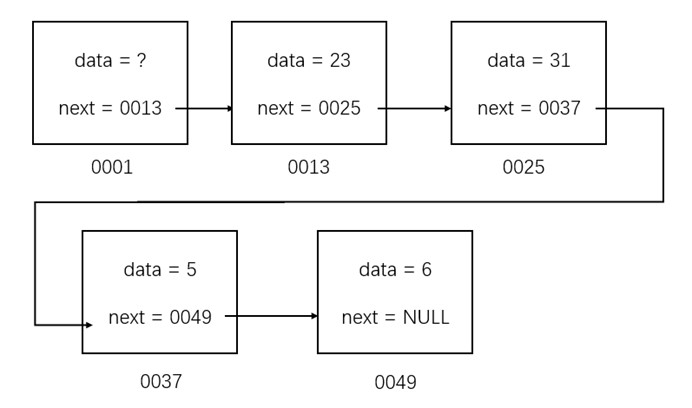
\includegraphics[width=0.6\textwidth,keepaspectratio]{picture/4.1.jpg}
\end{figure}

如上图所示,可以看到各个数据用指针next串成了一条链,因此这种数据结构称为\textbf{链表}。

链表中的每个数据也叫做\textbf{节点}。第一个节点叫\textbf{头节点},在程序中一般用指针head表示,一般情况下,头节点不存储数据(这是为了减少后续操作要考虑的特殊情况,比如删除链表中的某一个数,不会把头节点删掉)。

链表中的最后一个节点的next指针为NULL,因为没有后一个数。

在程序中定义指针 *p=head ,然后不断执行 p = p -\textgreater next 操作,直到p == NULL,就能让p遍历整个链表。

\subsection{\textcolor{blue}{链表的操作}}
\subsubsection{链表的建立}
开始时,链表中没有数据,只有一个不储存数据的头节点 head。
head -\textgreater data不需要管,因为head不存储数据(最好是初始化成问题中不会涉及到的数据,比如如果题目中只包含自然数则初始化成-1)。
head -\textgreater next为NULL,因为没有后一个数。

下面的Makelist()函数申请了一块内存并将next赋值为NULL,然后把这块内存地址返回给head
\begin{lstlisting}[language=C++,escapeinside={\%*}{*}]
struct link* Makelist()
{
	struct link *p = new struct link;
	p->next = NULL;
	return p;
}
//下面几行在main函数中 
struct link *head = NULL;
head = Makelist();
\end{lstlisting}
\subsubsection{链表插入节点}
在某个节点后插入数:
如下图,要在23后面插入78。
\begin{figure}[H]
	\centering
	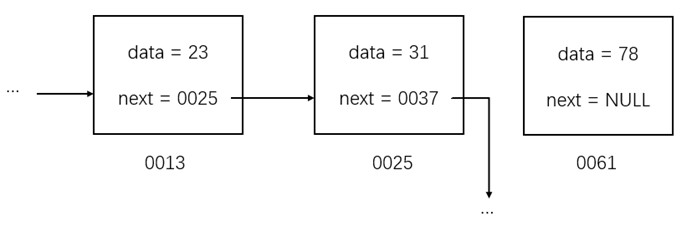
\includegraphics[width=0.6\textwidth,keepaspectratio]{picture/5.1.jpg}
\end{figure}
先将78的next指针指向0025(23的next指针)
\begin{figure}[H]
	\centering
	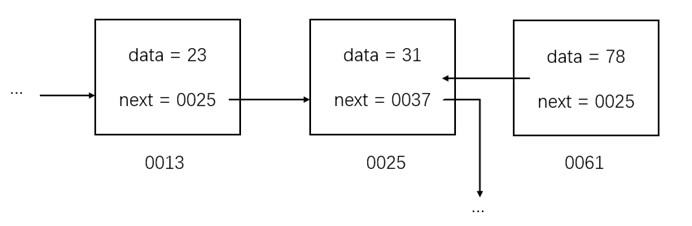
\includegraphics[width=0.6\textwidth,keepaspectratio]{picture/6.1.jpg}
\end{figure}
再把23的next指针指向0061(78的地址)
\begin{figure}[H]
	\centering
	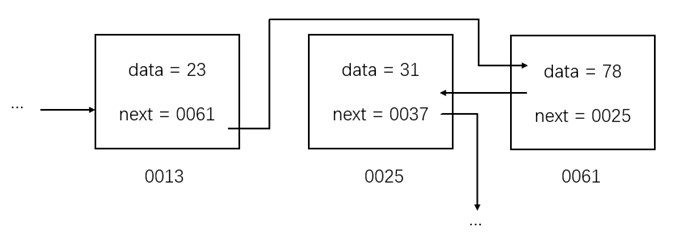
\includegraphics[width=0.6\textwidth,keepaspectratio]{picture/7.1.jpg}
\end{figure}
这就完成了78的插入
下面的函数实现了将数x插入到节点p后面的过程。
\begin{lstlisting}[language=C++,escapeinside={\%*}{*}]
void insert(struct link *p,int x)
{
	struct link *p1 = new struct link;
	p1->data = x;
	p1->next = p->next;
	p->next = p1;
}
\end{lstlisting}
在某个数x所在的节点后插入数y:
先用search函数(search函数的实现方法会在下面提到,先假设我们能写出一个函数search找到数x所在的节点)找到x所在的节点p(如果有重复,则找到的是第一个)。在节点p后插入数y即可。
\begin{lstlisting}[language=C++,escapeinside={\%*}{*}]
//在main函数中
cin >> x >> y;
struct link *p = search(head,x);
if(p!=NULL) insert(p,y);
\end{lstlisting}
\subsubsection{链表的查找}
查找数x所在的节点(如果有重复就是数x所在的第一个节点,以下不赘述):

定义指针 *p=head ,然后不断执行 p = p -\textgreater next 操作,让p遍历整个链表,找到x时返回p,遍历完还没找到则返回NULL。

下面的函数实现了查找数x所在节点的过程。
\begin{lstlisting}[language=C++,escapeinside={\%*}{*}]
struct link* search(struct link *head,int x)
{
	struct link *p = head->next;
	while(p!=NULL)
	{
		if(p->data == x) return p;
		p=p->next;
	}
	return NULL;
}
\end{lstlisting}
查找数x所在节点的前一个节点(下面讲删除的时候会用到):

在上面的代码中增加一个指针pre,始终指向p的前一个节点,找到x时返回pre即可。
\begin{lstlisting}[language=C++,escapeinside={\%*}{*}]
struct link* search_pre(struct link *head,int x)
{
	struct link *p = head->next, *pre = head;
	while(p!=NULL)
	{
		if(p->data == x) return pre;
		pre = p;
		p = p->next;
	}
	return NULL;
}
\end{lstlisting}
\subsubsection{链表删除节点}
删除某个节点:

如下图,要删除31(0025)
\begin{figure}[H]
	\centering
	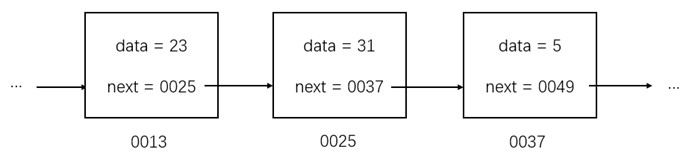
\includegraphics[width=0.6\textwidth,keepaspectratio]{picture/8.1.jpg}
\end{figure}
先将23(31的前一个节点)的next指针改为0037(31的next指针)
\begin{figure}[H]
	\centering
	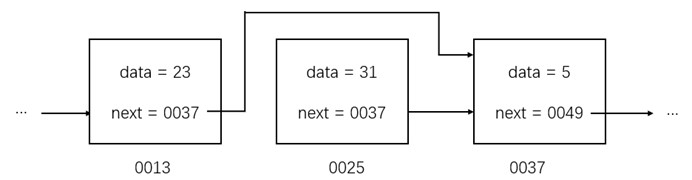
\includegraphics[width=0.6\textwidth,keepaspectratio]{picture/9.1.jpg}
\end{figure}
然后delete 0025,回收内存。
\begin{figure}[H]
	\centering
	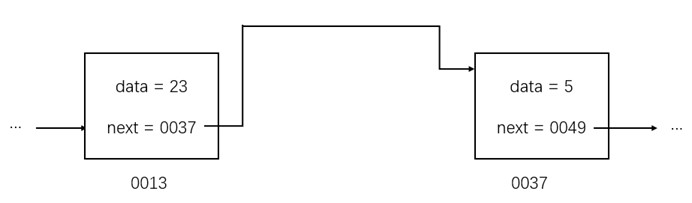
\includegraphics[width=0.6\textwidth,keepaspectratio]{picture/10.1.jpg}
\end{figure}

以下代码实现了删除p的后一个节点(注意是p的后一个节点):
\begin{lstlisting}[language=C++,escapeinside={\%*}{*}]
void remove_next(struct link *p)
{
	struct link *p1=p->next;
	if(p1==NULL) return; 
	p->next = p1->next;
	delete p1;
}
\end{lstlisting}
删除某个数x所在的节点:

用$search_pre$函数找到x所在节点的前一个节点p,并用$remove_next$函数把p的后一个节点(就是x所在的节点)删除.
\begin{lstlisting}[language=C++,escapeinside={\%*}{*}]
cin>>x;
struct link *p = search_pre(head,x);
remove_next(p);
\end{lstlisting}
\subsubsection{数据有序插入}
链表数据从小到大排列,要求插入数x后链表数据仍从小到大排列。

先找到链表中小于等于x的最后一个数,在这个数对应的节点后插入x。前一个操作可以对$search_pre$函数进行简单修改来完成。将返回条件修改为p -\textgreater data \textgreater x,并将最后一行由return NULL;改为return pre;(当找到比x大的数据节点时前一个节点pre即为所求,若没有找到,则循环结束时,p==NULL,pre为链表最后一个节点,也是所求节点)。后一个操作直接用insert函数进行。
\begin{lstlisting}[language=C++,escapeinside={\%*}{*}]
struct link* search_numpre(struct link *head,int x)
{
	struct link *p = head->next, *pre = head;
	while(p!=NULL)
	{
		if(p->data > x) return pre;
		pre = p;
		p = p->next;
	}
	return pre;
}
//在main函数中
cin>>x;
link *p=search_numpre(head,x);
insert(p,x);
\end{lstlisting}
\subsubsection{链表输出}
用一个指针p遍历链表的每个节点,依次输出数据即可。
\begin{lstlisting}[language=C++,escapeinside={\%*}{*}]
void print(struct link *head)
{
	struct link *p=head->next;
	while(p!=NULL)
	{
		cout<< p->data <<" ";
		p=p->next;
	}
	cout<<endl;
}

\end{lstlisting}


\section{栈、队列和排序}
\subsection{栈(Stack)}
\subsubsection{栈的基本概念}
栈是一种后进先出(LIFO, Last In First Out)的线性数据结构(可以先将数据结构视为可以完成\textbf{某些特殊操作的数据存储方式}),插入和删除操作仅在一端(栈顶)进行。(\textbf{栈类似于超市货物架,数据相当于商品},货架靠里的商品最先放进去,但最后被购买;相反,货架最外面的商品最后被放到货架上,但是最先被购买)
\begin{figure*}[htbp]
	\centering
	\begin{minipage}{0.49\linewidth}
		\centering
		
\includegraphics{picture/1.jpg}
	\end{minipage}
	\begin{minipage}{0.49\linewidth}
		\centering
		
\includegraphics{picture/2.jpg}
	\end{minipage}
\end{figure*}
\subsubsection{栈的基本操作}
\begin{itemize}
\item 初始化栈
\item 入栈(Push):将元素加入栈顶
\item 出栈(Pop):移除栈顶元素
\item 获取栈顶元素
\item 判断栈是否为空
\item 判断栈是否已满

\item 在c++语言STL库中提供了<stack>库,其中提供了push()、pop()等函数可以直接使用,本文不展开讨论\textbf{(注意期末考试能否使用\textless{}stack\textgreater{}需要依据老师要求!}
\item 单调栈是一种栈中元素单调排列的特殊栈,可以快速解决类似于“以某个值为最值得最大区间”等问题,本文不展开讨论
\end{itemize}
\subsubsection{\textcolor{blue}{栈的实现}}
以下是使用C++实现顺序栈的代码实现:
\begin{lstlisting}[language=C++,escapeinside={\%*}{*}]
include <iostream>
using namespace std;
#define maxn 1000

class Stack
{
	private://
	int stack[maxn];
	int top;
	public:
	Stack() { top = -1; } // 构造函数
	bool isEmpty() { return top==-1; }  // 判断是否为空
	bool isFull() { return top==maxn-1; }  // 判断是否已满
	void push(int x)  // 压入元素
	{
		if (isFull()) cout << "Stack Overflow.";
		else stack[++top] = x;
		return;
	}
	bool pop()  // 弹出元素
	{
		if (isEmpty()) cout << "Stack Underflow.";
		else top--;
		return;
	}
	int peek()  // 获取栈顶元素
	{
		if (isEmpty())
		{
			cout << "Stack is empty.";
			return -1;
		}
		else return stack[top];
	}
};
\end{lstlisting}
\subsubsection{\textcolor{blue}{栈的应用}}
括号配对\textbf{(2023-2024第一学期·程序设计基础期末考试)}:输入一串全部由括号组成的字符串,例如“( ( [ ] { } ) )”等。请判断这一串字符中的括号是否正确匹配;同时要求在括号匹配成功的条件下,字符串中不能出现小括号包含中括号、大括号,中括号内包含大括号的情况。

输入输出样例:

\begin{tabular}{|c|c|}
	\hline
	输入 & 输出 \\
	\hline
	\verb|(([]{}))| & No \\
	\verb|(([{]]))| & No \\
	\verb|{{[]()}}| & Yes \\
	\hline
\end{tabular}

问题解答:

问题分析:问题主要分为两部分:检查括号是否配对与检查是否有括号“递增”包含的情况。第一,检查括号是否配对可以通过栈在遍历字符串的过程中快速完成:在遍历过程中,如果当前的字符是左括号,则将其压入栈中;如果当前的字符是右括号,检查当前栈顶元素是否是与该右括号匹配。如果匹配,则将栈顶元素弹出,继续判断下一个字符;如果不匹配,则括号匹配失败。在遍历完整个字符串后,检查栈是否为空,若为空,则说明所有括号匹配成功,否则匹配失败。第二,检查是否有括号“递增”包含的情况,注意到,如果出现括号“递增”包含的情况,则一定存在\textbf{相邻的两个左括号},使得这两个左括号以\textbf{“递增形式”排列},因此,出现这种情况说明原字符串一定不符合要求。

%代码实现(下面的代码中直接使用了上述栈的实现代码,并将其中的int类型数组换为char类型数组):

\begin{lstlisting}[language=C++,escapeinside={\%*}{*}]
#include <iostream>
#include <string>
#include "Stack"
using namespace std;

int f(char ch);  // 将括号转变为数字
int main()
{
	string bracket;
	cin >> bracket;
	
	Stack s;
	int i;
	for (i=0; i<bracket.size(); i++)
	{
		if (f(bracket[i])>0)
		{
			if (!s.isEmpty() && f(bracket[i])>f(s.peek()))
			break;
			else s.push(bracket[i]);    
		}
		else
		{
			if (f(bracket[i])+f(s.peek())==0)
			s.pop();
			else break;    
		}
	}
	if (i!=bracket.size() || !s.isEmpty())
	cout << "No";
	else cout << "Yes";
	
	return 0;
}
\end{lstlisting}
\subsection{队列(Queue)}
\subsubsection{队列的基本概念}
队列是一种先进先出(FIFO, First In First Out)的线性数据结构,插入操作在队尾,删除操作在队首(顾名思义,队列中的数据操作与现实中排队类似。排队时,后来的人只能排在队尾,只有每一时刻排在队伍首端的人才能行动)(值得注意的是,\textbf{去年的期末考试以及日常课程中几乎没有涉及到队列},故就复习而言,队列并不是重点)。
\begin{figure}[htbp]
	\centering
	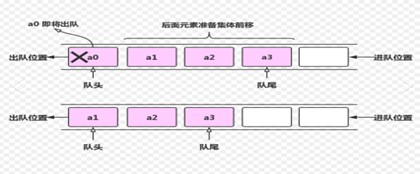
\includegraphics[width=0.77\textwidth]{picture/3.jpg}
\end{figure}
\subsubsection{队列的基本操作}
\begin{itemize}
\item 初始化队列
\item 入队(Enqueue):将元素加入队尾
\item 出队(Dequeue):移除队首元素
\item 获取队首元素
\item 判断队列是否为空
\item 在c++语言中STL库中提供了\textless queue\textgreater 库,其中有push()、front()函数可以直接使用,本文不展开讨论(\textbf{注意期末考试能否使用\textless queue\textgreater 需要依据老师要求!})
\item 单调队列可以快速解决类似于“区间内最值”等问题,本文不展开讨论
\item 单调队列是一种可以维护数据中最大或最小值得,可以在O(1)时间内获取数据中的最大值或是最小值,其底层数据结构为堆,\textless queue\textgreater 中\verb|priority_queue|就实现了优先队列的各种细节,本文不展开讨论。
\end{itemize}
\subsubsection{\textcolor{blue}{队列的实现}}
以下是使用C++实现链式队列的代码实现:
\begin{lstlisting}[language=C++,escapeinside={\%*}{*}]
#include <iostream>
using namespace std;

class Queue
{
	private:
	struct node
	{
		int data;
		node* next;
	};
	node* front;  // 队列头
	node* rear;  // 队列尾
	public:
	Queue() { front = rear = NULL; }  // 构造函数
	bool isEmpty() { return front == NULL; }  // 判断是否为空
	void Enqueue(int x)  // 插入元素
	{
		node* temp = new node;
		temp->data = x;
		temp->next = NULL;
		if (isEmpty()) front = rear = temp;
		else
		{
			rear->next = temp;
			rear = temp;
		}
	}
	void Dequeue()  // 删除元素
	{
		if (isEmpty())
		{
			cout << "Queue underflow.";
			return;
		}
		node* temp = front;
		front = front->next;
		delete temp;
	}
	int front()  // 获取队列头元素
	{
		if (isEmpty())
		{
			cout << "Queue is empty.";
			return -1;
		}
		return front->data;
	}
};
\end{lstlisting}
\subsubsection{\textcolor{blue}{队列的应用}}
舞会配对问题:在一场盛大的舞会中,有一些舞者已经排好队想要进行配对,他们当中有男有女,希望能够找出至少一种配对方法使得一男一女互相作为舞伴顺利参加舞会,请设计算法解决问题,输入的数组中0表示男,1表示女,输出中给出一种正确的配对方式,以数组元素下标数对的形式呈现,如果不能正确配对,输出-1。

输入输出样例:

\begin{tabular}{|l|l|}
	\hline
	输入 & 输出 \\
	\hline
	14 & 1 4 \\
	0 0 0 1 1 0 1 1 0 1 0 1 0 1 & 2 5 \\
	 & 3 7 \\
	 & 6 8 \\
	 & 9 10 \\
	 & 11 12 \\
	 & 13 14 \\
	\hline
	10 & -1 \\
	0 1 0 1 1 1 0 0 1 1 &  \\
	\hline
	\end{tabular}

问题解决:

问题分析:这是一道较为容易的分类配对问题,只需要先将男女舞者分为两类,之后从两类中逐个取出舞者进行配对即可。最后男女舞者数量不相等则显然无法正确配对。显然,从两类中分别取出舞者是一个典型的排队过程,可以使用队列模拟该过程。

具体代码实现(下面的代码使用了上述队列的实现代码):
\begin{lstlisting}[language=C++,escapeinside={\%*}{*}]
#include <iostream>
#include "Queue"
using namespace std;

int main()
{
	int n;
	cin >> n;
	int* dancer = int[n];
	for (int i=0; i<n; i++) cin >> dancer[i];
	int man=0,woman=0;
	Queue male;
	Queue female;
	for (int i=0; i<n; i++)
	{
		if (dancer[i]==0) 
		{
			male.Enqueue(i+1);
			man++;
		}
		else 
		{
			female.Enqueue(i+1);
			woman++;
		}
	}
	
	if (man != woman)
	{
		cout << "-1";
		return 0;
	}
	
	while (!male.isEmpty() && !female.isEmpty())
	{
		cout << male.front() << " " << female.front() << '\n';
		male.Dequeue();
		female.Dequeue();
	}
	
	return 0;
}

\end{lstlisting}
\subsection{排序(Sorting)}
\subsubsection{排序的基本概念}
排序是将一组数据按照某种标准进行有序排列。
\subsubsection{\textcolor{blue}{简单排序算法}}
下面的排序算法都以将整数数组升序排列为例,对于不能直接比较大小的元素类型需要首先自定义函数实现比较操作。(https://b23.tv/ru2YUYu,可以在这个视频中看到排序算法可视化的过程,有助于掌握不同排序算法)
\begin{itemize}
\item 冒泡排序(Bubble Sort)

冒泡排序的基本思想是通过不断遍历整个数组,每一次的遍历过程都将不断减少相邻逆序对的数量,最终减少为0。

关于冒泡排序,有一个简单的优化方法:如果在一次遍历过程中,没有发生过交换,则说明此时数组已经排序完成,退出循环即可。下面是代码实现:
\begin{lstlisting}[language=C++,escapeinside={\%*}{*}]
	void Bubble_Sort(int* arr, int n)
	{
		for (int i=0; i<n-1; i++)
		{
			int flag = 0;  // 优化:判断这一次遍历是否有交换
			for (int j=0; j<n-1-i; j++)
			{	
				if (arr[j]>arr[j+1])
				{
					flag = 1;
					int temp = arr[j];
					arr[j+1] = arr[j];
					arr[j] = temp;
				}
			}
			if (!flag) break;  // 没有发生交换,排序已经完成
		}
		return;
	}
	
\end{lstlisting}
\item 选择排序(Selection Sort)

选择排序的基本思想是在数组中未排序的部分中选出最小的元素,并将起放在以排序部分的尾部。下面是代码实现:
\begin{lstlisting}[language=C++,escapeinside={\%*}{*}]
void Selection_Sort(int* arr, int n)
{
	for (int i=0; i<n-1; i++)  // i代表未排序部分的第一个元素下标
	{
		int minIndex = i;
		for (int j=i; j<n; j++)
		{
			if (arr[j] < arr[minIndex])
			minIndex = j;
		}
		// 插入到已排序部分尾部
		int temp = arr[i];
		arr[i] = arr[minIndex];
		arr[minIndex] = temp;
		return;
	}

\end{lstlisting}
\item 选择排序(Selection Sort)

选择排序的基本思想是在数组中未排序的部分中选出最小的元素,并将起放在以排序部分的尾部。下面是代码实现:
\begin{lstlisting}[language=C++,escapeinside={\%*}{*}]
void Selection_Sort(int* arr, int n)
{
	for (int i=0; i<n-1; i++)  // i代表未排序部分的第一个元素下标
	{
		int minIndex = i;
		for (int j=i; j<n; j++)
		{
			if (arr[j] < arr[minIndex])
			minIndex = j;
		}
		// 插入到已排序部分尾部
		int temp = arr[i];
		arr[i] = arr[minIndex];
		arr[minIndex] = temp;
		return;
	}
\end{lstlisting}
\item 插入排序(Insertion Sort)

插入排序的基本思想是将未排序部分的元素逐一插入到已排序部分的正确位置,始终确保已排序部分的有序性。下面是代码实现:
\begin{lstlisting}[language=C++,escapeinside={\%*}{*}]
void Insertion_Sort(int* arr, int n)
{
	for (int i=1; i<n; i++)  // 认为arr[0]是已排好序的 
	{
		int key = arr[i];  // 未排序部分的第一个元素
		int j=i-1;
		while (j>=0 && arr[j]>key)
		{
			arr[j+1] = arr[j];
			j--;
		}
		a[j+1] = key;
	}
	return;
}

\end{lstlisting}
\end{itemize}
\subsubsection{“特殊”的排序}
\begin{itemize}
\item 高级排序(高级排序在去年的程序设计基础课程和考核中\textbf{几乎没有涉及})

高级排序有很多种,不难证明,前文中提及到的简单排序算法的平均时间复杂度都是$O(n^2)$,
而高级排序的平均时间复杂度为$O(nlogn)$。高级排序有很多种,例如归并排序、堆排序、快速排序等。本文主要介绍快速排序。快速排序的基本思想是“分治”,即将问题分为一个个子问题分而治之。具体来说,首先\textbf{任意选取一个元素作为枢纽},扫描数组将元素重新排列,使得枢纽“左端”的元素不大于枢纽,枢纽“右端”的元素不小于枢纽,需要注意的是,这里\textbf{只要求分布正确,不要求直接排好序}。此时,对原数组进行排序的问题就转化为了对枢纽左、右侧分别进行排序的两个子问题,对这两个数组重复上述步骤即可(需要使用递归函数)。下面是具体的算法实现:
\begin{lstlisting}[language=C++,escapeinside={\%*}{*}]
void Fast_Sort(int* arr, int left, int right)
{
	if (left == right) return;
	
	int mid = (left+right)/2;
	int pivot = arr[mid];  // 选择枢纽
	int i=left,j=right;
	while(i<j)
	{
		while(arr[i]<=pivot)
		i++;
		while(arr[j]>=pivot)
		j--;
		int temp = arr[i];
		arr[i] = arr[j];
		arr[j] = temp;    
	}
	FastSort(arr,left,mid);
	FastSort(arr,mid+1,right);
	return;
}
\end{lstlisting}
\item 有序序列的快速合并\textbf{(2022-2023第一学期·程序设计基础期末考试)}

现在给出两个已经按递增顺序排好序的数组,请设计算法,在尽可能短的时间内将两个数组合并为一个数组,且合并后的数组需要仍然保持有序(会根据算法运行时间给分,时间过长会有一定程度的扣分)。


输入输出样例:

\begin{tabular}{|l|l|}
	\hline
	输入 & 输出 \\
	\hline
	4 5 // 两个数组的元素个数 & 1 2 3 4 6 7 8 9 11 \\
	1 2 4 8 & \\
	3 6 7 9 11 & \\
	\hline
\end{tabular}

问题解答:

问题分析:为充分利用两个数组已经排好序的性质,对于两个数组一边比较、一边选择而逐个取出元素进行合并。具体到示例中的两个数组来说,先比较1和3,1较小,将1放入“合数组”中;比较2和3,2较小,将2放入“合数组”中;比较4和3,3较小,将3放入“合数组”中;比较4和6......易见这种合并方法可以达到线性时间复杂度,且常数为1,是能做到的最优时间复杂度。

具体代码实现:
\begin{lstlisting}[language=C++,escapeinside={\%*}{*}]
#include <iostream>
using namespace std;

int main()
{
	int n,m;
	cin >> n >> m;
	int* arr1 = new int[n];
	int* arr2 = new int[m];
	for (int i=0; i<n; i++) cin >> arr1[i];
	for (int i=0; i<m; i++) cin >> arr2[i];
	
	int i=0,j=0,k=0;
	int* arr = new int[n+m];
	while (i<n && j<m)
	{
		if (arr1[i]<arr2[j]) arr[k++] = arr1[i++];
		else arr[k++] = arr2[j++];
	}
	
	if (i==n)
	for (; j<m; j++,k++) arr[k] = arr2[j];
	else
	for (; i<n; i++,k++) arr[k] = arr1[i];
	
	for (int t=0; t<n+m; t++) cout << arr[t] << " ";
	return 0;
}

\end{lstlisting}
\end{itemize}

\section{面向对象的程序设计(蓝色为重点章节)}
\subsection{何为面向对象的编程}
\subsubsection{面向对象与面向过程}
在了解面向对象的编程前,先了解一下面向过程的编程。面向过程,指我们先分析出解决问题所需要的步骤,然后用函数把这些步骤一步一步实现,使用的时候一个一个依次调用。在学习面向对象之前,我们编写的所有程序均是面向过程的。

举个例子,在游戏飞机大战中,要实现飞机发射子弹消灭敌机的功能,大致包含以下步骤:子弹发射、子弹飞行、子弹命中、敌机消失。对于每一步,我们都可以编写相应的函数实现对应功能。
\begin{figure}[H]
	\centering
	
\includegraphics[width=0.25\textwidth,keepaspectratio]{picture/11.jpg}
	\caption{飞机大战}
\end{figure}
那么何为面向对象的编程?

还是以飞机大战为例,游戏中存在许多的敌机。如果使用面向过程的编程实现敌机,我们需要定义一个结构体存储敌机的数据,再分别实现敌机运动,发射子弹,被消灭等函数,之后在主函数中依次调用。如果只有一架敌机,上述步骤很容易完成。但在游戏中存在多种敌机,每种敌机不止一架且总是在生成新的。

如果每生成一架都要重新在主函数中调用上述函数,太过于麻烦。我们希望将敌机的数据及它的函数打包成一个整体,每次创建敌机就调用这个整体,传入不同的参数就生成不同的敌机,之后这些敌机自行调用自己的函数来运动或攻击,直至消失。

这就是面向对象的编程。在面向对象的编程中,我们把事物都抽象为“对象”,每个对象都可以拥有它的属性(数据)与行为(函数)。我们就可以通过调用这些对象的方法、属性去解决问题。
\subsubsection{\textcolor{blue}{基本概念}}
对象:对象是由数据(描述事物的属性)和作用于数据的操作(体现事物的行为)组成的封装体,描述客观事物的一个实体。例如在上述例子中,每个生成的敌机都是一个对象。

类:类是对一组有相同数据和相同操作的对象的定义,是对象的模板,其包含的方法和数据描述一组对象的共同行为和属性。例如上述例子中,敌机的数据与其函数共同构成了敌机类,根据这个类,我们可以创建出一个一个的敌机。

由此可见,类好比是对象的蓝图(抽象),而对象是根据类这个蓝图生产出的产品(具体)。
\subsubsection{基本特征:封装、继承、多态}
封装即信息隐蔽。它是指在确定系统的某一部分内容时,应考虑到其它部分的信息及联系都在这一部分的内部进行,外部各部分之间的信息联系应尽可能的少。

具体表现为我们将尽可能多的信息隐藏起来,只对外提供有限的接口用于访问。例如在上述例子中,敌机类只提供了创建敌机的接口,但是敌机的速度、位置,子弹的发射时间都隐藏在内部,无法从外部直接访问上述数据。

在c++中,访问修饰符private将变量声明为私有变量,外部无法访问(相对的,public将变量声明为公有变量,可以从外部访问)。

继承:让某个类型的对象获得另一个类型的对象的属性和方法。继承就是子类继承父类的特征和行为,使得子类对象(实例)具有父类的实例域和方法,或子类从父类继承方法,使得子类具有父类相同的行为。

多态:对于同一个行为,不同的子类对象具有不同的表现形式。多态存在的3个条件:1)继承 2)重写 3)父类引用指向子类对象。

对于多态和继承的解释在后面完成。
\subsection{面向对象编程的基本语法}
\subsubsection{\textcolor{blue}{类 、数据成员与成员函数}}
类是创建对象的蓝图,包含数据成员和成员函数。数据成员是类的属性,用于存储对象的状态。成员函数是类的方法,用于定义可以对对象执行的操作。

在c++中,类的关键词为class。类的声明方式如下。
\begin{lstlisting}[language=C++,escapeinside={\%*}{*}]
class Person {
	public:
	std::string name; // 数据成员
	void introduce() { // 成员函数
		std::cout << "My name is " << name << std::endl;
	}
};
\end{lstlisting}
这里定义了一个名为Person的类,它有一个公共数据成员name和一个公共成员函数introduce。name用于存储人的名字,introduce函数用于输出这个人的名字。

此外还可用如下方式声明成员函数。
\begin{lstlisting}[language=C++,escapeinside={\%*}{*}]
class Person {
	public:
	std::string name; // 数据成员
	void introduce(); // 成员函数
};

void Person::introduce() {
	std::cout << "My name is " << name << std::endl;
}
\end{lstlisting}
\subsubsection{\textcolor{blue}{对象}}
对象是类的实例,使用类名后跟对象名来创建。
\begin{lstlisting}[language=C++,escapeinside={\%*}{*}]
Person person1; // 创建Person类的对象
\end{lstlisting}
这行代码创建了Person类的一个实例(对象),名为person1。
\subsubsection{\textcolor{blue}{构造函数}}
调用person1的introduce方法,输出为My name is,并没有输出名字。这是因为没有编写构造函数,编译器提供默认构造函数将name赋为空,需编写构造函数初始化对象。构造函数没有返回类型。

你也可以定义自己的默认构造函数而不用编译器给出的版本。但是\textbf{如果你定义了非默认构造函数,如果还想使用默认构造函数,则一定要定义默认构造函数,否则会报错}。实现如下。
\begin{lstlisting}[language=C++,escapeinside={\%*}{*}]
class Person {
	public:
	Person(std::string n){
		name = n;
	} // 非默认构造函数
	Person(){
		name = "ji xin qin";
	} // 默认构造函数。如果定义了非默认构造函数,不定义直接使用会报错
	// 如果没有定义非默认构造函数,编译器会给出默认构造函数,不定义直接使用不会报错
	std::string name; // 数据成员
};

int main (){
	string m="jxq";
	Person person1; // 调用默认构造函数
	Person person3(m); // 调用非默认构造函数
}
\end{lstlisting}
上述声明还可写为以下形式:当调用默认构造函数时(不向构造函数中传入参数),此时n的值为给定的“ji xin qin”。当调用非默认构造函数时,n的值为传入的参数。之后name(n)语句将n的值赋给name,完成对象的构造。
\begin{lstlisting}[language=C++,escapeinside={\%*}{*}]
class Person {
	public:
	Person(std::string n = "ji xin qin") : name(n){}
	std::string name; // 数据成员
};
\end{lstlisting}
拷贝构造函数:一种特殊的构造函数,接受一个对象并将它复制一遍,产生一个新的对象。如果自己没有定义,编译器会给出默认版本。但如果成员变量包含指针,务必自行编写拷贝构造函数进行深拷贝。(原因见后面)
\begin{lstlisting}[language=C++,escapeinside={\%*}{*}]
Person b(a);//将a传入拷贝构造函数,得到a的拷贝b
\end{lstlisting}
深拷贝与浅拷贝:

浅拷贝是指在复制对象时,只复制对象的顶层数据,而不复制对象内部指向的动态分配的内存。对于对象内部的指针成员,浅拷贝只复制指针的值,而不是指针指向的数据。因此,新对象和原对象会共享相同的内存空间。
\begin{lstlisting}[language=C++,escapeinside={\%*}{*}]
int a[]={1,2,3};
int *b = a;       //b为a的浅拷贝(两个指针指向同一片空间)
\end{lstlisting}
深拷贝是指在复制对象时,不仅复制对象的顶层数据,还复制对象内部指向的所有动态分配的内存。对于对象内部的指针成员,深拷贝会为新对象分配新的内存,并复制指针指向的数据。
\begin{lstlisting}[language=C++,escapeinside={\%*}{*}]
int a[]={1,2,3};
int *b = new int[3];       
for(int i=0;i<3;i++) b[i] = a[i];
//b为a的深拷贝(两个指针指向不同空间)
\end{lstlisting}
\subsubsection{\textcolor{blue}{析构函数}}
析构函数用于对象销毁时的清理工作,与类同名,以波浪号开头,没有返回类型。(如果没用使用动态内存分配,则无需编写析构函数,编译器自动给出的版本就很好。)
\begin{lstlisting}[language=C++,escapeinside={\%*}{*}]
class Person {
	public:
	int *a;
	Person(int n){
		a = new int[n];
	}
	Person(){
		a = NULL;
	}
	~Person(){
		if(a!=NULL)
		delete [] a;
	} // 调用析构函数释放掉a
};
\end{lstlisting}
\subsubsection{\textcolor{blue}{访问修饰符}}
public:公共部分可以被任何代码访问。

private:私有部分只能被类自己的成员函数访问。

(课内用的少)protected:保护部分可以被类自己的成员函数和派生类访问。

\textcolor{blue}{(考试中千万不要图方便将题目中的private改为public,被发现了会扣很多分)}
\subsubsection{\textcolor{blue}{对象数组}}
指每一个数组元素都是对象的数组。访问方式和访问其他类型的数组一样。初始化方式与访问方式如下。
\begin{lstlisting}[language=C++,escapeinside={\%*}{*}]
class Person {
	public:
	std::string name;
	int age;
	Person(std::string n, int a)  {
		name = n, age = a;
	}    // 构造函数
	Person(){
		name = "jxq", age = 114514;
	}
	void display(){ cout<<name<<' '<<age;}
};
int main() {
	Person people[5]; // 使用默认构造函数初始化所有元素
	
	Person people2[] = {
		Person("Li Tiansuo", 24),
		Person("Chun Ping", 37),
		Person("Van", 52)
	}; // 列表初始化
	Person people3[5];
	for (int i = 0; i < 5; i++) {
		people3[i] = Person("Name" + std::to_string(i), 24);
	} //使用循环
	people2[0].display(); //下标访问
	//运行结果 Li Tiansuo 24
}
\end{lstlisting}
\subsubsection{\textcolor{blue}{this指针}}
上述成员函数均只涉及一个对象。但是要完成某些任务,需要设计包含多个对象的成员函数。例如我想比较两个person对象的年龄(name变量)的大小,就需要一个包含两个对象的成员函数:
\begin{lstlisting}[language=C++,escapeinside={\%*}{*}]
Person & compare(Person& b){ //调用一个对象的成员函数,传入另一个对象的引用,返回年龄较大对象的引用
	if(age<=b.age)
		return b; //返回另一个对象的引用
	else 
		return ???; //如何返回自身的引用
}
\end{lstlisting}
编写该成员函数时,当自身的年龄较大时需返回自身,但是我们不知道该如何称呼自身。这时需用到this指针。this指针指向当前对象自身,*this即为自身的引用。
\begin{lstlisting}[language=C++,escapeinside={\%*}{*}]
Person & compare(Person& b){ //调用一个对象的成员函数,传入另一个对象的引用,返回年龄较大对象的引用
	if(age<=b.age)
		return b; //返回另一个对象的引用
	else 
		return *this; //返回自身的引用
}

Person people2[] = {
	Person("Li Tiansuo", 24),
	Person("Chun Ping", 37),
	Person("Van", 52)
}; // 列表初始化
Person older = people2[0].compare(people2[1]); //调用对象people2[0]的成员函数compare,传入参数people2[1]
older.display(); //输出为Chun Ping 37
\end{lstlisting}
同时我们会发现,涉及一个对象(自身)的成员函数不需要参数,而涉及两个对象的只需要一个参数。这是因为在成员函数中,另一个参数(对象自身)以this指针的形式隐式传入,无需再显式传入。
\subsubsection{关于引用}
在将对象传入函数时,一般以引用形式传递。这是因为如果按值传入,编译器会先调用拷贝构造函数,再将拷贝传入函数,在函数调用完毕后会自动调用析构函数删除拷贝。如果对象较大,这会产生很大的开销。而且在某些情况下,按引用传递可以防止程序出错(具体见《拷贝构造函数与动态内存分配》)。

在将变量(包括基本类型变量,如int double与自己定义的类的对象)传出函数时,\textcolor{blue}{如果该变量是以引用形式传入的,直接将该引用传出即可}。例如取大函数:
\begin{lstlisting}[language=C++,escapeinside={\%*}{*}]
int max(int &a, int &b){
	if(a>b)
	return a;
	else
	return b;
}
\end{lstlisting}
\textcolor{blue}{但是如果该变量是按值传入的或是在函数内部创建的变量,请直接按值返回}。这是因为这些变量都是函数的临时变量,当函数调用完毕时对应内存会被释放掉,无法再用引用访问它。例如
\begin{lstlisting}[language=C++,escapeinside={\%*}{*}]
int add(int &a, int &b){
	int c = a + b;
	return c; //不能写为return &c
}
\end{lstlisting}
\subsubsection{拷贝构造函数与动态内存分配}
先看如下代码
\begin{lstlisting}[language=C++,escapeinside={\%*}{*}]
#include<cstring>
#include<iostream>
using namespace std;

class Person {
	public:
	std::string name;
	int age;
	int kids; //孩子的个数
	int *kage;	 //存储孩子们的年龄
	Person(std::string na, int a, int n,int g[])  {
		name = na, age = a;
		kids = n;	
		kage = new int[n]; //存储孩子们的年龄,使用了动态内存分配
		for(int i=0;i<n;i++)
		kage[i] = g[i];		//将g的元素赋值给kage
	}    // 构造函数
	void display(){ 
		cout<<name<<' '<<age<<endl<<kids;
		for(int i=0;i<kids;i++) cout<<' '<<kage[i];
		cout<<endl;
	}		//输出person对象信息
	Person compare(Person b){ //调用一个对象的成员函数,传入另一个对象
		if(age<=b.age)
		return b; //返回另一个对象
		else 
		return *this; //返回自身
	}
	~Person(){
		delete [] kage;  //释放kage指针
	}
}; //不定义拷贝构造函数,使用编译器给出的版本
int main(){
	int g1[] = {2,5};
	int g2[] = {1,3,4};
	Person a("li",33,2,g1);
	Person b("cheng",34,3,g2);
	b.display(); //第一次调用b的display
	Person c = a.compare(b); //调用a的compare函数,将b以参数形式传入
	b.display(); //第二次调用b的display
	while(true){} //防止程序退出
}
\end{lstlisting}
输出为

cheng 34

3 1 3 4 (第一次)

cheng 34

3 1465199521 5 489219044  (第二次)

两次调用b的display,我们没有改变b的值,结果却不同。这是因为没有定义拷贝构造函数,编译器会为你提供一个默认的拷贝构造函数,这个默认的拷贝构造函数会进行浅拷贝。也就是说,它会复制对象的成员变量,但对于指针类型的成员变量,它只会复制指针的值,而不是指针指向的内存块。这将导致两个 Person 对象(b和 compare 函数中的临时对象)的 kage 指针指向同一块内存。当 compare 函数结束后,它的局部对象被销毁,kage 指针指向的内存被释放。再次调用b的display将无法得到正确结果。

(当 main 函数结束时,b对象也被销毁,kage 指针指向的内存再次被释放,这会导致 double free 错误。为了演示输出,要阻止程序退出)

此时需要自己定义拷贝构造函数进行深拷贝。
\begin{lstlisting}[language=C++,escapeinside={\%*}{*}]
    Person(const Person &p) {
	name = p.name;
	age = p.age;
	kids = p.kids;
	kage = new int[kids];   //创建新的kage指针,指向另一片新的空间
	for (int i = 0; i < kids; i++)
	kage[i] = p.kage[i];    //深拷贝
}   // 深拷贝构造函数
\end{lstlisting}
但对于上述例子,如果compare函数为按引用传入参数,可以规避调用拷贝构造函数创建临时对象,减小程序开销,也可避免发生错误。

\textcolor{blue}{简要总结:用动态内存分配时请务必自己定义深拷贝的拷贝构造函数,同时对象传入函数时按引用传递。}
\subsection{\textcolor{blue}{运算符重载}}
运算符重载是面向对象编程语言中的一种特性,它允许程序员为自定义的数据类型(类或结构体)定义或改变已有的运算符(如 +、-、*、/ 等)的行为。通过运算符重载,可以使得自定义类型的操作更加直观和自然,类似于内置类型。

通过重载运算符,可以实现多态行为,使得不同类型的对象可以使用相同的运算符进行操作。

例如,我们定义了一个复数类,想用加号实现复数相加。但是c++并没有内置这样的操作,直接用会报错。因此我们需要重载加号,实现对复数类的相加。语法为:
返回类型  operator+(传入参数){函数体}

(加号可换为其他想要重载的运算符,例如可换为 >,重载 >用于比较两个复数的模)
\begin{lstlisting}[language=C++,escapeinside={\%*}{*}]
#include<iostream>
#include<cmath>
using namespace std;
class Complex {
	public:
	double real, imag;
	Complex(double r = 0.0, double i = 0.0) : real(r), imag(i) {}
	
	// 重载加法运算符
	Complex operator+(const Complex& other) const {
		return Complex(real + other.real, imag + other.imag);
	}  
	void display(){
		cout<<'('<<real<<','<<imag<<')'<<endl;
	}
	// 计算复数的模
	double magnitude() const {
		return sqrt(pow(real, 2) + pow(imag, 2));
	}
	// 重载>运算符
	bool operator>(const Complex& other) const {
		return this->magnitude() > other.magnitude();
		//也可写为return magnitude() > other.magnitude();
	}
};
int main() {
	Complex c1(2, 3), c2(4, 5);
	Complex c3 = c1 + c2;
	c3.display(); // 输出:(6,8)
	if (c1 > c2) c1.display();
	else c2.display();
	//输出:(4,5)
	return 0;
}
\end{lstlisting}
事实上, a + b等价于a.operator+(b), a + b是标准的运算符使用方式。当你使用 a + b 时,编译器会在 a 对象上查找 operator+ 函数,并以 b 作为参数调用它。如果 a 的类型没有定义 operator+(),则编译器会尝试使用 b 的类型定义的 operator+()(如果 b 是非内置类型),或者使用内置的加法运算符。可以认为运算符重载就是重写了operator+()这个函数,为两个Complex变量提供了加号方法。

使用加法需要前后两个参数,但是在以成员函数重载时我们只提供了后一个,前一个以this指针隐式传入。

由此可见我们也可以再次重载加号,使其能完成复数与实数(double类型)的相加,重载代码如下:
\begin{lstlisting}[language=C++,escapeinside={\%*}{*}]
    Complex operator+(double num) const {
	return Complex(real + num, imag);
}
\end{lstlisting}
但是在使用时我们发现,相加只能写成: 复数 + 实数
的形式,写成  实数 + 复数 的形式则会报错,提示no match for ‘operator+’ (operand types are ‘double’ and ‘Complex’)。

这是因为在C++中,运算符重载是不可逆的,这意味着如果我们用成员函数重载了 Complex 类的 operator+ 来实现复数与实数的加法,我们不能直接使用 operator+ 来实现实数与复数的加法,因为编译器会根据操作数的类型来决定使用哪个 operator+ 函数。

同时,我们也不能直接重载基本数据类型(如 double、int 等)的运算符。

由此可见,我们无法像之前那样使用this指针隐式传入参数,两个参数均需要显式传入。需要定义接受两个参数的非成员函数,前一个参数为double类型,后一个为Complex对象。

函数原型为:
\begin{lstlisting}[language=C++,escapeinside={\%*}{*}]
   Complex operator+(double num, const Complex& c) {
	return Complex(c.real + num, c.imag); 
}
\end{lstlisting}
但是如果成员变量real与imag被声明为私有成员变量,该函数无法执行,因为非成员函数无法直接访问私有成员变量。因此需要将该函数声明为友元函数。

\textcolor{blue}{友元函数}

在C++中,友元函数是一种特殊的非成员函数,它被赋予了访问权限,可以访问类的私有(private)和保护(protected)成员(包含成员变量与成员函数)。尽管友元函数不属于类的成员函数,但它与类的关系非常紧密,因为它可以访问类的内部实现细节。

友元函数在类中声明,使用关键字friend,例如上述函数可被声明为:
\begin{lstlisting}[language=C++,escapeinside={\%*}{*}]
   friend Complex operator+(double num, const Complex& c) {
	return Complex(c.real + num, c.imag); 
}
\end{lstlisting}
由此我们实现了实数与复数的相加。

利用友元函数,我们还可以实现其他运算符的重载,如重载$<<$,使cout可以输出Complex类对象。

cout 是ostream类的对象,在ostream类中,c++重载了位运算符 << ,使cout对象可以用其输出int char等类型的变量。我们也可以进一步重载<<,使cout可以输出Complex类对象。示例代码如下:
\begin{lstlisting}[language=C++,escapeinside={\%*}{*}]
     friend ostream& operator<<(ostream& os, const Complex& c) 	{ 	//函数的返回类型为ostream&,用于连续输出
	
	//函数接受两个参数,一个是ostream类对象的引用os,以及需要输出的Complex类对象
	
	os << "(" << c.real << ", " << c.imag << ")"; 			  //os为ostream对象的引用,此处等同于cout
	return os;  	//返回os,用于连续输出
}
\end{lstlisting}
也可以用相同的方法重载cin(istream类型对象)与$>>$。

Complex类完整代码如下:
\begin{lstlisting}[language=C++,escapeinside={\%*}{*}]
#include <iostream>
using namespace std;
class Complex {
	private:
	double real, imag;
	public:
	Complex(double r = 0.0, double i = 0.0) : real(r), imag(i) {}
	
	Complex operator+(const Complex& other) const {
		return Complex(real + other.real, imag + other.imag);
	}	//成员函数 重载+用于计算两个复数相加
	Complex operator+(const double num){
		return Complex(real + num, imag);
	} //成员函数 重载+用于计算复数与实数相加
	friend Complex operator+(double num, const Complex& c) {
		return Complex(c.real + num, c.imag); 
	}	//友元函数 重载+用于计算实数与复数相加
	friend ostream& operator<<(ostream& os, const Complex& c) { 
		os << "(" << c.real << ", " << c.imag << ")"; 
		return os; 
	} //友元函数 重载 << 用于输出复数
};
int main() {
	Complex c1(2, 3);
	double num1 = 5.5;
	double num2 = 2.3;
	Complex c2 = c1 + num1;
	Complex c3 = num2 + c1;
	cout << "c1 + num1: " << c2 << endl; //运行结果 c1 + num1: (7.5, 3)
	cout << "c1 + num2: " << c3 << endl; //运行结果 c1 + num2: (4.3, 3)
	return 0;
}
\end{lstlisting}
拓展:
\begin{lstlisting}[language=C++,escapeinside={\%*}{*}]
#include <iostream>
using namespace std;
class Complex {
	private:
	double real, imag;
	public:
	Complex(double r = 0.0, double i = 0.0) : real(r), imag(i) {}
	
	Complex operator+(const Complex& other) const {
		return Complex(real + other.real, imag + other.imag);
	} //成员函数重载+用于计算两个复数相加
	friend Complex operator+(double num, const Complex& c) {
		return Complex(c.real + num, c.imag); 
	} //友元函数重载+用于计算实数与复数相加
	friend ostream& operator<<(ostream& os, const Complex& c) { 
		os << "(" << c.real << ", " << c.imag << ")"; 
		return os; 
	} //友元函数重载 << 用于输出复数
};
int main() {
	Complex c1(2, 3);
	double num1 = 5.5;
	float num2 = 2.3;
	int num3 = 3;
	Complex c2 = c1 + num1;
	Complex c3 = c1 + num2;
	Complex c4 = num3 + c1 ;
	cout << "c1 + num1: " << c2 << endl;
	cout << "c1 + num2: " << c3 << endl;
	cout << "c1 + num3: " << c4 << endl;
	return 0;
}
\end{lstlisting}
在上述代码中,我并没有定义复数加实数的情况,同时实数的类型仅为double,没有定义int与float类型的重载,却没有报错,同时得到正确结果。感兴趣的同学可以去查一查为什么(编译器实在是太智能了)。

这种做法并不推荐,可能会影响性能,因为涉及到临时对象的创建,并且可能会使代码的意图不够明确。明确重载所有相关的运算符是更好的选择,以提高代码的可读性和可维护性。

\textcolor{red}{但是将double,int,float对应的重载函数全写出来太过繁琐,也不符合代码重用的原则,为此需要使用模板。我们将在后续的篇章中介绍模板的使用。}


\textcolor{blue}{赋值运算符的重载:}

参考拷贝构造函数,当自己未定义时,编译器会自动给出浅拷贝的版本。\textcolor{blue}{当成员变量中包含指针时(存在动态内存分配),则需要自己编写深拷贝版本。(原因是为了防止浅拷贝导致两个对象的指针指向同一片空间,进而导致double free等错误,详细原因见 《拷贝构造函数与动态内存分配》 章节)}实现例子如下:
\begin{lstlisting}[language=C++,escapeinside={\%*}{*}]
 class Person {
	private:
	std::string name;
	int age;
	int kids;
	int *kage;
	public:
	
	Person(std::string na, int a, int n,int g[])  {
		name = na, age = a;
		kids = n;
		kage = new int[n];
		for(int i=0;i<n;i++)
		kage[i] = g[i];
	}    // 构造函数
	
	Person(const Person &p) {
		name = p.name;
		age = p.age;
		kids = p.kids;
		kage = new int[kids];   
		for (int i = 0; i < kids; i++)
		kage[i] = p.kage[i];    //深拷贝
	}   // 深拷贝构造函数
	
	Person& operator=(const Person &p) {
		if (this != &p) { // 防止自赋值,例如语句为p=p时直接返回,不执行后续代码
			delete [] kage; // 释放原有的动态数组,如果是自赋值,此处会删除自身kage数组,导致后续赋值操作出错。
			name = p.name;
			age = p.age;
			kids = p.kids;
			kage = new int[kids];
			for (int i = 0; i < kids; i++)
			kage[i] = p.kage[i];
		}
		return *this;  //返回自身引用,用于连续赋值
	}
};
\end{lstlisting}
\subsection{函数的cv限定}
注明: 这里的cv限定是指const限定和volatile限定,而后者并不在本材料的讨论范围内(亦不在考纲内),因而以下着重关注const限定,但适用于const限定的语法也使用于volatile限定。

类的非静态成员函数可以带有cv限定符(const,volatile,const和volatile组合三种),这些限定符在形参列表之后、函数体(对定义)/分号(对声明)之前.具有不同的限定符(包括无限定)的,具有相同名字和相同形参列表的函数,被视作不同函数,因而可以相互重载,唯他们的返回类型必须相同(即仍然适用不允许仅有返回类型不同的函数重载的规则).语法如同:
\begin{lstlisting}[language=C++,escapeinside={\%*}{*}]
class MyClass{    
	private:        
	int member1;        
	int member2;    
	public:        
	void const_func() const {}
};
\end{lstlisting}
在有cv限定符的函数体内,指针*this有同样的cv限定.换句话说,在函数带有const限定符后,在函数体内不能修改类的任何(非mutable)成员的值,同时也只能调用同一类中同样带有const限定符的那些成员函数(即不能调用同类中不带有const限定的函数,即便这些函数实际上不会修改成员值),否则是编译错误。

函数的const限定版本通常用于const对象的调用.因为const对象也不允许修改其成员值,因而只能调用函数的const版本.但是非const对象也能调用const版本,因而一个常用的实践是:\textbf{假如某函数的实际意义保证不会修改成员的值,那么将他声明为const的}。

上述实践的特例是,该函数是集访问和修改于一体的,那么这时最好声明一个无限定版本的、一个带const限定版本的,例如重载数组下标访问运算符:
\begin{lstlisting}[language=C++,escapeinside={\%*}{*}]
#include <vector> 
class Array{   
	public:
	std::vector<int> data;    
	Array(int sz) : data(sz) {}     
	// const 成员函数    
	int operator[](int idx) const    {          // this 指针具有类型 const Array*        
		return data[idx];       // 变换为 (*this).data[idx];    
	}                           
	// 非 const 成员函数    
	int& operator[](int idx){   // this 指针具有类型 Array*        
		return data[idx];       // 变换为 (*this).data[idx]    
	}
};
\end{lstlisting}
尤其需要注意,当返回到成员的指针/引用时,二者的cv限定要同函数的cv限定匹配,返回值则无此限制(const版本可以把返回值改为const int\&)。

在使用上面的类型时:
\begin{lstlisting}[language=C++,escapeinside={\%*}{*}]
int main(){    
	Array A(10); // 非const对象    
	const Array B(10); // const对象
	A[5] = 1; // 调用非const版本, 修改成功    
	(A[5]); // 调用非const版本, 即使未修改其值
	(B[5]); // 调用const版本    
	// B[5] = 2; 错误: const版本返回值,结果不是可修改左值
	const auto* p = &A;    
	((*p)[5]); // 调用const版本    
	// (*p)[5] = 3; 错误: 同上
	const auto& q = A;    
	(q[5]); // 调用const版本    
	// q[5] = 4; 错误: 同上

\end{lstlisting}
可见上述规则对通过指针和引用调用时也适用。

\large \textbf{mutable成员}

有时候我们想让类的某个成员总是可变,无论调用方是否为const对象,这时可以声明该成员为mutable的。

形式化地说,mutable说明符可出现在类的非静态、非常量、非引用成员的声明中:
\begin{lstlisting}[language=C++,escapeinside={\%*}{*}]
class Student{  
	public:  
	string Name;    
	string ID;    
	mutable int grade;
	Student(string a = "jxq", string b = "0721", int c=2): Name(a), ID(b), grade(c){}
	//  static mutable string school; 
	// 错误: 不允许出现在静态成员声明中
	//  mutable const int grade; 
	// 错误: 不允许出现在常量声明中
	//  mutable int& deskmate; 
	// 错误: 不允许出现在引用声明中
};
\end{lstlisting}
则即使有对象const Student stu;:
\begin{lstlisting}[language=C++,escapeinside={\%*}{*}]
int main(){    
	const Student stu("luotianyi","0712",1);    
	stu.grade++; // 成功, mutable成员总是可变
	//  stu.Name = "XJTU"; 
	// 失败
	//  stu.ID = "66CCFF"; 
	// 失败
}
\end{lstlisting}
上述过程亦同样可用在带const限定的成员函数之中,用来修改mutable成员的值,例子略。
\subsection{类继承}
还是以游戏飞机大战为例。对于我们的战机、敌机、飞行的子弹这三种对象(三个类),他们都是飞行的物体,能向前或向后运动。因此对于这三个类,我们都需要编写对应的运动函数以及碰撞检测函数,但是这些函数本质上都是相同的,编写三遍不符合代码重用原则,也容易出错。

由此我们想到:考虑到它们三个都是飞行的物体,能不能创建一个描述飞行的物体的基类,然后以此为基础,添加三者自己特有的功能,创建出三个派生类。这样三者共有的运动函数以及碰撞检测函数均只用编写一次,同时如果将来还要加入其他运动的物体(比如炸弹),也只需要在此基础上添加对应功能即可。

上述方法便是类继承,它可以让我们在已有类的基础上添加新的功能、变量或修改原类的行为。继承有助于将代码组织成层次结构,使得代码更加模块化,易于理解和维护。

\subsubsection{\textcolor{blue}{类继承基本语法(公有继承)}}
类继承的一种常见情况是:a是一种b(‘a’ is a kind of ‘b’),我们称这种关系为is-a关系,可由b派生得到a。例如学生是人,我们可用person类(基类)派生出student类(派生类)。派生类的声明方式如下:
\begin{lstlisting}[language = C,basicstyle=\small\ttfamily]
class Person {
private:
    int age; // 私有成员变量 age

public:
    // 构造函数
    Person(int a=24) : age(a) {}
    // 公有函数 display 展示年龄
    void display() {
        cout << "Age: " << age << endl;
   }
}; //person基类

class Student : public Person {

}; //派生类声明

int main (){
    Student a;
    a.display(); //输出Age: 24
}
\end{lstlisting}

虽然我们没有为派生类编写任何函数,但是上述代码依然能输出。这是因为Student 类是继承自 Person 类的。它自动继承了 Person 类的所有公有成员和保护成员。这意味着 Student 类的对象可以直接访问 Person 类的公有成员函数,包括 display() 函数。同时由于 Student 类没有自己的构造函数,编译器会自动调用基类 Person 的构造函数来初始化对象,因此a的值为24。

现在我们为student类添加它自己的变量、构造函数与display函数。
    
在编写student类的构造函数以及重写display函数时,我们发现age作为Person类的私有成员变量,我们无法直接访问。同时相同的赋值及输出代码再写一遍也不符合代码重用原则。因此我们希望使用到Person类的构造函数与display函数。具体代码如下:
\begin{lstlisting}[language = C,basicstyle=\small\ttfamily]
class Student : public Person {
private:
    int grade; // 私有成员变量 grade

public:
    // 构造函数。使用Person(a),以a为参数调用Person的构造函数,将age的值初始化为a
    Student(int a=0, int g=0) : Person(a), grade(g) {} 
    // 公有函数 display 展示年龄与年级
void display() {
    // 调用基类的 display 函数,语法为: 基类名+::(域操作符)+函数名
        Person::display(); 
        cout << "Grade: " << grade << endl;
    }
};

int main() {
    // 创建 Student 对象
     Student student1(20, 10);
     Student student2;
     student1.display(); // 展示年龄与年级
     student2.display();
     return 0;
}
\end{lstlisting}

但是并不是所有的关系都是is-a关系,还有has a关系(例如午餐中含有水果,但是午餐不是水果)、use a关系(吃午餐用筷子,但筷子不是午餐,午餐也不是筷子)、is like a关系(冰箱与衣柜有相似之处,但是冰箱不是衣柜,衣柜也不是冰箱)和is implement as a关系(栈可以用数组实现,但是栈不是数组(无法下标访问))。 描述上述关系的方法超出了本材料讨论范围,同学们可以自行查阅。

\subsubsection{多次继承}
一个类可以同时继承自多个基类,只要用逗号将基类名称隔开,并且要为每个基类指明public/private/protected继承(注:见下几节)。

\subsubsection{\textcolor{blue}{多态继承}}
\paragraph{静态类型和动态类型}静态类型是指对程序进行编译分析时,所得到表达式的类型。相对应的概念是动态类型:如果某个指针或者引用指向一个多态对象(派生类对象),那么其最终派生对象为其动态类型。

以下是一个简单的例子:
\begin{lstlisting}[language = C,basicstyle=\small\ttfamily]
struct Base { virtual ~Base() {} };
struct Derived : Base {};
Derived ObjectDerived; // 最终派生对象Base ObjectBase;
Base *P1 = &ObjectDerived; // (*P1) 的静态类型为Base, 因P1是Base型指针// (*P1) 的动态类型为Derived, 因其指向一个派生类对象
Base *P2 = &ObjectBase;// (*P1) 的静态类型为Base, 动态类型也是Base
\end{lstlisting}

\paragraph{引入多态继承的目的}
虽然派生类和基类之间的关系是IS-A关系,即派生类对象是一个基类。因此可以直接使用基类指针或引用指向派生类对象。但有些时候,在派生类中某个基类方法和基类中的行为不完全一样,但又想通过一种方法统一管理基类对象和派生类对象,这就需要引入多态继承。

首先来看一个直观的想法,直接通过基类指针试图调用派生类方法:
\begin{lstlisting}[language = C,basicstyle=\small\ttfamily]
#include<bits/stdc++.h>
using namespace std;
struct Student{    
private:    
    string Name;    
    string ID;
public:    
    void print()    
    {        
        cout<<"Name: "<<Name<<endl;        cout<<"ID: "<<ID<<endl;
    }
};
struct InternationalStudent : Student{   
    string National;
    void print()    
    {        
        Student::print(); // 必须使用域解析作用符,否则陷入递归cout<<"National: "<<National<<endl;    
    }
};
int main(){    // 创建同时含有基类和派生类的数组    
    vector<Student*> Stus;     for(int i = 0; i < 10; i++) 
    {        
        if(i&1)
            Stus.push_back(new Student);      
        else 
            Stus.push_back(new InternationalStudent);
    }
    for(size_t i = 0; i < Stus.size(); i++)     
    {        
        Stus.at(i) -> print();
    }
    // ...
}
\end{lstlisting}
上述代码能不能实现预期目标:编译器根据指针指向对象的动态类型来调用对应方法?答案是否定的,Stus.at(i)->print();一句永远只能调用基类方法,也就是说,即使输入的学生是个InternationalStudent,也不会打印其国籍。

在上述代码前提下,C++没有提供方法判断对象动态类型,即使是dynamic\verb|_|cast和typeid也要求类型是多态的.一个取巧的方法是,假如知道该数组的奇数位是基类类型,偶数位是派生类类型,那么可以直接使用(无运行时类型检查)强制类型转换来搞定这件事:
\begin{lstlisting}[language = C,basicstyle=\small\ttfamily]
int main(){    // ...  
    for(size_t i = 0; i < Stus.size(); i++) {        
        if(i&1){            
            Stus[i] -> print();// 已经判断为基类类型  
        }      
        else{ 
            static_cast<InternationalStudent*>(Stus[i])->print();  // 或(InternationalStudent*)(Stus[i])->print();        
        }    
    }    // ...
}
\end{lstlisting}

这种方法并不推荐,因为他有几个严重的问题:

1.必须已知哪些元素是基类对象而哪些是派生类对象;

2.如果不小心对基类对象作强制类型转换并且解引用,就会导致未定义行为;

3.在析构(使用delete)时,必须重新进行判断,否则就会调用基类析构函数,造成"派生类"部分资源的内存泄露。

\paragraph{引入多态}
使用virtual函数说明符,能将类的非静态成员函数声明为一个虚函数,使得该函数的行为可以在派生类中被覆盖,或者说,当通过基类指针或引用调用该函数时,编译器根据他们所指对象的动态类型调用该类型中的对应实现,称最终调用的版本为最终覆盖函数.一个类被称为多态的,当其含有至少一个虚成员函数.基于多态类的继承叫做多态继承.
virtual函数说明符一般放在返回类型前面,但其实他们的顺序可以是任意的:
\begin{lstlisting}[language = C,basicstyle=\small\ttfamily]
#include<bits/stdc++.h>
using namespace std;
struct Student{    
    string Name;   
    string ID;
    virtual void print() // void virtual print()也ok    
    {        
        cout<<"Name: "<<Name<<endl;        
        cout<<"ID: "<<ID<<endl;    
    }    
    virtual ~Student() {}
};
struct InternationalStudent : Student{   
    string National;
    void print(){        
        Student::print();        
        cout<<"National: "<<National<<endl;    
    }    
    ~InternationalStudent() {}
};
int main(){    
    // 创建同时含有基类和派生类的数组    
    vector<Student*> Stus;     
    for(int i = 0; i < 10; i++){        
        if(i&1)    Stus.push_back(new Student);        
        else   Stus.push_back(new InternationalStudent);    
    }
    for(size_t i = 0; i < Stus.size(); i++){        
        Stus.at(i) -> print(); // 将根据Stus[i]的实际类型调用    
    }
    for(size_t i = 0; i < Stus.size(); i++){        
    delete Stus[i];    
    }
}
\end{lstlisting}

在上述例子中,基类的print函数和析构函数被声明为虚,那么就可以在遍历时通过基类指针调用这两个函数:

1.对于动态类型为Student的对象,调用基类的print()和~Student()。

2.对于动态类型为InternationalStudent的对象,调用派生类的print()和~InternationalStudent()。

\subsubsection{\textcolor{blue}{细节}}
\paragraph{派生类中的虚函数}
注意到,我们在派生类中没有声明print为虚的,这是因为当基类的某个函数vf是虚函数时,派生类的函数自动成为虚函数并且将覆盖vf,无论其声明中是否出现virtual,当且仅当其满足如下四个条件:

1.名字相同,即也为vf

2.形参列表(不是返回类型)

3.const限定符 // volatile限定符

4.// 引用限定符

注:带//标记的行是不在考纲范围内的内容,但为列举严谨性而写出.在考试出现的所有内容中均可以当作这些要求不存在,下同。

这说明,如果在基类中重载了某个虚函数,要想在派生类中使用覆盖他们,就必须为每个想要覆盖的函数写出实现(其他函数会被隐藏,见"不满足函数覆盖的情形")

\paragraph{析构函数}
析构函数是个特例,只要底层基类的析构函数是虚的,那么派生类的析构函数也是虚的。若底层基类的析构函数非虚,那么试图通过基类指针删除派生类对象是未定义行为,即使这样做不会造成资源泄露。一个常用的方针是:要么基类的析构函数是public且virtual的,要么是protected且非virtual的.后者可以保证不能通过基类指针删除派生类对象(而必须通过派生类对象本身或其指针或其引用调用派生类的析构函数)

\paragraph{最终覆盖函数}
如果派生类中没有能覆盖底层基类中vf的函数(包括在派生类中声明和通过多重继承得到的候选函数),那么底层基类中的vf就是最终覆盖函数。

\paragraph{返回类型要求}
上面的要求中并没有提到返回类型,是因为对返回类型有特别要求:若基类中某个函数vf是虚函数,而派生类中声明了满足上述四个条件的函数,那么两个函数的返回类型要么是相同的,要么是协变的,否则是编译错误。

若基类vf返回类型T1和派生类vf返回类型T2满足以下要求,则他们协变(Covariance):

1.两个类型都是到类类型的单级指针或引用(// 都为左值引用或都为右值引用.)

2.T1所指向(或被引用,下同)的类,必须是T2所指向的类的无歧义可访问的直接或间接基类。

3.T2必须较T1拥有同等或更少的const(// volatile)限定。

也就是说,T1所指向的类在继承层级上的关系要比T2所指向的类更"基层"。

例如,如果在不改变基类函数声明的情况下,将InternationalStudent中的函数声明修改成

int print(){    // ...    return 1;}

就会编译不通过,报错大意为:覆盖函数的返回类型与基类类型既不相同,也不协变。

插入一句完全的题外话,在除了main函数之外的所有有返回值函数中,语句执行到最后而没有return语句是未定义行为,即便调用方无需获取其值.在严格编译环境下(treat all warnings as errors)会抛出编译错误,在其他情况下可能会导致程序出现错误结果.因此必须保证函数末尾有一句return语句。

\paragraph{有限定名字查找 vs 无限定名字查找}
有限定名字查找,即函数名出现在作用域解析运算符::的右侧时,明确指明调用某个函数时使用哪一个版本(相对于调用者静态类型的直接或间接基类中各实现中的一个,且可以为其本身),其语法为:对象名/基类引用.基类名::函数名(参数列表)基类指针->基类名::函数名(参数列表)以下是一个例子:

\begin{lstlisting}[language = C,basicstyle=\small\ttfamily]
// 类的定义省略
int main(){   
InternationalStudent IStu;    
Student *pStu = &IStu;    
Student &rStu =  IStu;
// 虚调用    
pStu->print(); // 派生类版本,打印国籍    
rStu.print(); // 派生类版本,打印国籍
// 非虚调用    
pStu->Student::print(); // 基类版本,不打印国籍   
rStu.Student::print(); // 基类版本,不打印国籍
// 通过对象直接调用    
IStu.Student::print(); // 基类版本,不打印国籍}
\end{lstlisting}

否则是无限定名字查找,这时应用虚调用。

\paragraph{不满足函数覆盖的情形}
若名字相同但形参列表不同,且基类函数为虚:不覆盖基类函数,但隐藏基类函数。通过基类指针调用时,始终调用基类版本(派生类版本不可见,试图调用派生类版本是编译错误);通过派生类对象或其指针/引用调用时,始终调用派生类版本(基类版本不可见,试图调用基类版本是编译错误,唯通过有限定名字查找方式调用则仍成功)。

若一个函数拥有不止一个最终覆盖函数,那么是编译错误:
\begin{lstlisting}[language = C,basicstyle=\small\ttfamily]
struct A{   
    virtual void f();
};
struct D1 : A{    
    void f(); // 覆盖A::f()
};
struct D2 : A{    
    void f(); // 覆蓋A::f()
};
struct D : D1, D2{}
\end{lstlisting}

以上代码中D同时从D1和D2两个地方继承了函数void f(),并且他们互不覆盖,这样编译器无法确定要使用哪一个,就会抛出二义性错误。

\paragraph{构造函数}
构造函数不允许是虚的。派生类创建对象时,先调用派生类的构造函数,在执行其函数体前,通过成员初始化列表调用基类的构造函数。这是一种调用,而非继承,也就是说派生类构造函数无意覆盖基类的构造函数,不需要也不能把基类构造函数设置为虚。

\paragraph{友元}
virtual关键字只能用于类的非静态成员函数。友元函数不是成员函数,因而不能为虚。但此方面设计问题可透过在友元中调用虚函数来解决。

\subsubsection{\textcolor{blue}{静态联编和动态联编}}
\paragraph{指针和引用的向上转换和向下转换}
一般来说,C++不允许(隐式地)将除了空指针常量之外的一种类型的地址赋给另一类型的指针,亦不允许使用一种类型的引用指向另一种类型.即使使用显式转换这样做了,也不能安全地解引用转换后的指针.但由于派生类中包含了(至少)一个完整的基类,因而可以使用基类指针或引用指向派生类对象而无需使用强制类型转换,这种隐式类型转换叫做向上强制转换(upcasting).相对应地,将基类指针或引用转换为派生类指针或引用称为向下强制转换(downcasting).此转换必须通过强制(显式)类型转换完成.一种常用的手段是使用dynamic\verb|_|cast,该转换能安全地沿着继承层级向上,向下及侧向转换指针和引用.注意,该手段要求多态继承。

这里仅仅简要地列出dynamic\verb|_|cast<目标类型指针或引用类型>(待转换指针/引用)的常见用法:
\begin{lstlisting}[language = C,basicstyle=\small\ttfamily]
struct Base{ 
    virtual void f() {} 
};
struct Derived : Base {};
int main(){    
    Derived D;    
    Base B;   
    Base *ptrB1 = &D;   
    Base *ptrB2 = &B;
    if( dynamic_cast<Derived*>(ptrB1) ) // 成功转换    
    {        
    Derived *ptrD = dynamic_cast<Derived*>(ptrB1); // 拿到派生类指针    
    }    
    if( dynamic_cast<Derived*>(ptrB2) ) // 转换失败返回空指针,隐式转换到false    
    {        // 不会执行    
    }
}
\end{lstlisting}

当指针转换失败时,会返回目标类型的空指针值,这会经过bool隐式转换到false,因而判断会失败.当引用转换时,会抛出std::bad\verb|_|cast错误,需要使用try-catch块捕捉异常。

\paragraph{静态联编 动态联编}
编译器将源代码中函数调用与函数代码绑定的过程称为函数名联编.对于一般函数,函数名和形参列表就足以在编译时完成这一任务,这种方式被称为静态联编.但对于虚函数,由于在编译时,编译器无法确定调用方的动态类型,因而无法确定应调用哪个版本的函数,因而确定调用哪个函数将需要在运行时完成,这种方法被称为动态联编.编译器对虚调用使用动态联编,对非虚调用使用静态联编。

为什么动态联编不是默认行为?因为动态联编会引入虚函数表(内存开销),在运行时决定调用哪个函数会带来时间开销.当某类无需用作基类或某函数在派生类中无需覆盖时,没有必要使用动态联编.因而按照C++的设计原则,在确实需要这样做的时候才使用虚函数和动态联编。

\paragraph{虚函数表}
一种常见的动态联编实现是使用虚函数表.编译器为多态类中添加一个隐藏成员,该成员为一指向函数地址数组的指针,称该函数地址数组为虚函数表,虚函数表中储存了为类对象进行声明的虚函数的地址.每个多态类有自己的表.底层基类的虚函数表保存了其所有虚函数,派生类的虚函数表保存最终覆盖函数的地址(未覆盖的函数保存基类的地址,覆盖了的函数保存覆盖函数的地址),在派生类中新加入的虚函数亦被加入表中.调用虚函数时,程序查看储存在对象中的隐藏成员,转向相应的函数地址表.使用声明顺序的第几个虚函数,就调用函数地址表中的第几个函数。

使用g++编译时,加入编译指令-fdump-lang-class可以查看虚函数表。

\subsubsection{访问控制}
\paragraph{类的protected成员}
首先需要强调的是,在C++中,结构体关键字struct和类关键字class的作用完全一致,他们都声明一个类(可以有成员,构造函数等),除了以关键字struct声明的类的成员在不加注明的情况下是public的,以class声明的不加注明的情况下是private.同样地,以这两种关键字声明的类在继承中有完全一样的行为,除了以关键字struct声明的类在不加注明的情况下是public继承,以class声明的类在不加注明的情况下是private继承。

以下重温public成员和private成员的可见性,并引入protected可见性:

• public成员总是可见;

• private成员仅对同一个类的成员和友元可见,允许是同一个类的两个实例;

• protected成员允许以下两种情况的访问:

1.当前类的成员和友元;
2.派生自该类的任何类的成员和友元,但仅仅在通过该派生类或该派生类的派生类的对象访问时允许。

以下是来自cppreference的参考代码,解释了protected成员的特性:
\begin{lstlisting}[language = C,basicstyle=\small\ttfamily]
struct Base{
protected:    
    int i;
private:   
    void g(Base& b, struct Derived& d);
};
struct Derived : Base{    
friend void h(Base& b, Derived& d);    
void f(Base& b, Derived& d) // 派生类的成员函数    
    {        ++d.i;  // OK:d 的类型是 Derived        
             ++i;    // OK:隐含的 '*this' 的类型是 Derived//      
             ++b.i;  // 错误:不能通过 Base 访问受保护成员                
             // (否则可能更改另一派生类,假设为 Derived2 的基实现)    
    }
};
void Base::g(Base& b, Derived& d) // 基类的成员函数{    
    ++i;    // OK    
    ++b.i;  // OK   
    ++d.i;  // OK
}
void h(Base& b, Derived& d) // 派生类的友元{    
    ++d.i; // OK: 派生类的友元可以通过派生类的对象访问受保护成员// 
    ++b.i; // 错误: 派生类的友元并非基类的友元
}
void x(Base& b, Derived& d) // 非成员非友元{    
    ++b.i; // 错误:非成员不能访问 
    ++d.i; // 错误:非成员不能访问
}
\end{lstlisting}

\paragraph{public继承 private继承 protected继承}
这三种继承的语法如下:
\begin{lstlisting}[language = C,basicstyle=\small\ttfamily]
class Base { 
    public: 
        virtual void f() {}
};
class D1 : public Base {}; // public继承
class D2 : protected Base {}; // protected继承
class D3 : private Base {}; // private继承
\end{lstlisting}
三种继承的作用如下:
• 类使用 public 成员访问说明符从基类派生时,基类的所有公开成员可作为派生类的公开成员访问,基类的所有受保护成员可作为派生类的受保护成员访问(基类的私有成员始终不可访问,除非设为友元)。

• 当类使用 protected 成员访问说明符从基类派生时,基类的所有公开和受保护成员可作为派生类的受保护成员访问(基类的私有成员始终不可访问,除非设为友元)。

• 当类使用 private 成员访问说明符从基类派生时,基类的所有公开和受保护成员可作为派生类的私有成员访问(基类的私有成员始终不可访问,除非设为友元)。

公有继承最好地描述了is-a关系,无论继承多少层,派生类总是一个(always is-a)其直接或间接基类:经公有继承派生的派生类指针/引用总是能向上转换强制到基类指针/引用。

受保护继承其次,因为描述的关系是:在派生类成员,以及所有进一步派生的类中,派生类is-a基类,因而只有在派生类和派生类的派生类的成员内部,才能对派生类指针/引用向上强制转换到基类指针/引用。

私有继承最次,因为描述的关系是:在派生类成员中(而非进一步派生的类中),派生类is-a基类,因而只有在派生类的成员内部,才能对派生类指针/引用向上强制转换到基类指针/引用。

\subsubsection{\textcolor{blue}{抽象基类}}
抽象基类(Abstract Base Class, ABC)是为了解决不完美的is-a关系而存在的东西.请看下例:

现在有个椭圆类
\begin{lstlisting}[language = C,basicstyle=\small\ttfamily]
class Ellipse{    
    private:        
        double x; // 中心点坐标x 
        double y; // 中心点坐标y   
        double a; // 长半轴       
        double b; // 短半轴       
        double angle; // 长半轴与x轴正方向的夹角    
    public:        
        void Move(int xx, int yy) { x = xx, y = yy; }  
        virtual double Area() const { rturn 3.14159 * a * b; }
        virtual void Rotate(double newAngle){ angle = newAngle; }
}
\end{lstlisting}

显然圆是椭圆,但是使用多态公有继承会出现问题,逐个分析成员:

1.圆有x和y,这没有问题

2.圆无需使用a和b来描述其形状,因为a=b=r

3.圆没有角度,进而Rotate不应在圆中实现

4.圆的面积函数需要修改通过手段来隐藏这些不需要的内容不如重新写一个,但这样就放弃了他们的共性部分.

C++允许引入抽象基类来抽象出这样一个"共性部分",尽管他们没有任何物理意义.这样的共性部分可以包括属性和方法,进而通过继承来:

1.增添属性(例如a,b,r)

2.增添方法(例如Rotate函数)

3.为不同的派生提供同含义但实现不同的方法
(例如Area的不同实现)

首先,考虑共性部分:
\begin{lstlisting}[language = C,basicstyle=\small\ttfamily]
class BaseEllipse{    
    private:        
        double x; // 中心点坐标x  
        double y; // 中心点坐标y
    public:     
    BaseEllipse(double xx = 0, double yy = 0) : x(xx), y(yy) {}        
    virtual ~BaseEllipse() {}   
    void Move(int nx, int ny) { xx = nx, yy = ny; }
    virtual double Area() const = 0; 
} 
\end{lstlisting}
共性部分包括了x,y和具体的Move和一个抽象的Area,因为我们无法从已知参数求得Area.称形如Area函数为纯虚函数,其语法为

virtual 返回类型 函数名(形参列表) 可选cv限定 = 0; 

表示该函数留待派生类实现。

拥有至少一个纯虚函数的类称为抽象基类,由于这样的类通常没有物理意义,因而不允许创建抽象基类的对象,但仍允许使用其指针和引用指向其派生类。

这样就可以进而实现两个派生类:
\begin{lstlisting}[language = C,basicstyle=\small\ttfamily]
class Circle : public BaseEllipse {   
    private:       
        double r;    
    public:       
        Circle(double xx = 0, double yy = 0, double rr = 0) : BaseEllipse(xx, yy), r(rr) {}
        ~Circle() {}
        double Area(){
            return 3.14159 * r * r;       
        }
} 
class Ellipse : public BaseEllipse{    
    private:        
        double a;      
        double b;     
        double angle; 
    public: // 构造函数,析构函数留作练习
        double Area(){            return 3.14159 * a * b;
        }        
        double Rotate(double newAngle){
        angle = newAngle;
        }
}
\end{lstlisting}

关于纯虚函数的一个重要细节是:纯虚函数将在派生类层级中保持纯虚,直到某个派生类给出一个实现.也就是说,在某个派生类里,通过继承或定义方式得到的最终覆盖函数中有至少一个纯虚函数,该派生类就仍为抽象基类,不能构建该派生类的对象。

抽象基类的理念更像一种规范,他要求所有自其派生的类(要想使用的话)都至少实现了抽象基类的所有要求(尽管可以通过private+空实现来逃课。)
\paragraph{语法细节}
1.纯虚函数说明不能和定义(函数体)同时出现。

2.不能把友元声明为纯虚。

3.抽象类型不能作为形参类型,函数返回类型或显式类型转换的目标类型,以上检查在函数定义和调用点检查。

4.可以为纯虚函数提供定义(而且如果纯虚函数是析构函数就必须提供,因为在销毁派生类时,所有基类析构函数都会被调用):派生类的成员函数可以自由地用有限定的函数标识(::作用符)调用抽象基类的纯虚函数.此定义必须在类体之外提供(函数声明的语法不允许纯说明符=0和函数体一起出现)。

5.从抽象类的构造函数或析构函数中进行纯虚函数的虚调用是未定义行为(无论纯虚函数是否拥有定义)。

\subsubsection{\textcolor{blue}{继承和动态内存分配}}
\paragraph{析构顺序}
对于用户定义或隐式定义的析构函数,在析构函数体执行后,编译器会以声明的逆序调用该类的所有非静态(// 非变体)数据成员的析构函数,然后以构造的逆序调用所有直接(// 非虚)基类的析构函数(继而调用它的成员与它的基类的析构函数,以此类推).(// 最后,如果此对象类型是最终派生类,那么调用所有虚基类的析构函数.)上述规则在显式调用析构(Object.\verb|~|ClassName())时也应用。
\paragraph{派生类的析构}
由于上述规则的存在,无需在派生类析构函数函数体中对他的任何基类作出任何动作.如果派生类中没有新增的使用动态内存分配的成员,那么使用默认析构函数就可以.否则,必须为派生类提供析构函数定义,并且该定义中只需要处理派生类构造函数中那些使用动态内存分配的成员,而基类中那些动态内存分配的成员期望基类的析构函数能正确处理。
\paragraph{派生类的复制构造}
如果派生类中没有新增的使用动态内存分配的成员,那么使用默认复制构造函数就可以,因为默认行为会调用基类的复制构造函数,并将传入的派生类对象中的基类部分通过基类复制构造函数构造对象的基类部分;其他平凡成员通过各自的复制构造函数完成构造。

如果派生类中有新增的使用动态内存分配的成员,那么必须显式提供复制构造函数定义.同上,函数体中只需要处理派生类中那些使用动态内存分配的成员,而基类部分直接使用成员初始化列表完成(或省却这一步并调用基类的默认构造),平凡成员可选在成员初始化列表中或者在函数体内完成。

请注意,这里发生了从派生类引用到基类引用的向上转换,其语法类似

Derived(const Derived\& rhs) : Base(rhs){    // 正常处理动态内存分配的复制构造}

\paragraph{派生类的赋值构造运算符}
这里的赋值构造运算符是指复制赋值运算符,即为新对象重新开辟空间,旧对象依旧保持有效。

如果派生类中没有新增的使用动态内存分配的成员,那么使用默认赋值运算符就可以,因为默认行为会调用基类的赋值运算符,并将传入的派生类对象中的基类部分通过基类的赋值运算符赋值到调用方的基类部分,这期待基类的赋值运算符能够正确处理基类中各成员的复制;同时调用其他平凡成员各自的赋值运算符完成赋值。

如果派生类中有新增的使用动态内存分配的成员,那么必须显式提供复制构造函数定义.同上,定义中只需要处理派生类中的成员,而基类部分通过显式调用基类的赋值运算符完成.注意,要重新判断自赋值。其语法类似:
\begin{lstlisting}[language = C,basicstyle=\small\ttfamily]
struct Base{ 
    virtual void f() {} 
};
struct Derived : Base{ 
    Derived& operator=(const Derived& rhs){
        if(this == & rhs) return *this; // 处理基类        
    Base::operator=(rhs); // 处理其他派生类成员    
    }
};
\end{lstlisting}

题外话,标准库中提供的类都已经保证自赋值安全,在所使用成员中如果没有裸露的指针,可以省略自赋值检查。

\subsection{认识模板}
\subsubsection{什么是模板?}
模板是一个C++实体,其定义以下其一:

• 类模板: 一族类,可以是子类

• 函数模板: 一族函数,可以是成员函数

• // 别名模板: 一族类型的别名 (C++11起)

• // 变量模板: 一族变量 (C++14起)

• // 概念 (C++20起) 在教学及期末考试中只会涉及到类模板和函数模板,因而只会针对这两类模板展开叙述;为求严谨,在本节涉及到定义处会列举所有情况,即使他们不在考纲内,这部分内容以行注释标记。

对于上述定义中"一族"的定义,可以类比数学中的曲线系:

$(x-a)^2+(y-b)^2=C:a,b$为已知常数

定义了一簇曲线(一系列同心圆),当给定一个C的时候,上述方程转而指定一个特定的圆.模板也是这样,他拥有至少一个模板形参,进而表示一族类或者函数,当所有模板形参被指定时,类模板指定一个特定的类而函数模板指定一个特定的函数。

\subsubsection{\textcolor{blue}{声明模板}}
声明模板最简单的方式是使用template关键字,template关键字代表接下来要声明一个模板,紧随其后的尖括号内是模板形参序列,用以指定模板形参,模板形参分为以下三种

• 类型模板形参

• 非类型模板形参

• // 模板模板形参

一个模板形参序列可以是上述三种模板形参的随意组合,两个模板形参之间以逗号隔开。

使用typename关键字或class关键字声明的模板形参是类型模板形参,代表了这里需要填入一个类型,两个关键字在声明模板形参时作用完全一致,没有分别。
\begin{lstlisting}[language = C,basicstyle=\small\ttfamily]
template <typename T>
class MyClass{}; // 声明一个类模板MyClass

template <class T>
void MyFunc(); // 声明一个函数模板MyFunc
\end{lstlisting}

这种方式引入一个类型T,他是一个等待确定的类型(一如曲线系中的参数),该类型T被当作已知类型,并可以在声明的类模板或者函数模板中使用,例如用来声明成员等:
\begin{lstlisting}
template <typename T>
class Circle
{
    T radius; // 用T来声明一个成员
}

template <typename T>
T DoNothing(T a) // 用T来指定返回类型和函数参数类型
{
    return a; 
}
\end{lstlisting}

非类型模板形参则不同,他引入一个对象作为模板形参,该对象的类型可以是:

• 引用 (// 左值引用)

• 整数类型

• 指针类型

• 其他特定类型,详见\href{https://zh.cppreference.com/w/cpp/language/template_parameters}{模板形参与模板实参}

例如:
\begin{lstlisting}
template <unsigned int Size>
class Array{}; // 声明一个类模板Array
\end{lstlisting}

这时,在模板内可以视作已经定义了一个这样的变量Size,该变量不可修改(除非他是引用类型)。

将上面提到的两种模板形参综合起来,我们可以定义一个简单的模板类:
\begin{lstlisting}
template <typename T, unsigned int Size> // 一个类型模板形参,一个非类型模板实参
struct Array // Array是一个模板类
{
    T* pointer; // 声明一个类型为T*的指针作为成员

    Array() { pointer = new T[Size]; } 
    // 构造函数: 开辟一个能装下Size个T的内存并赋给pointer
    
    ~Array() { delete[] pointer; }
    // 析构函数: 将初始化时分配的内存回收.
};
\end{lstlisting}

\subsection{模板的实例化}
一个模板声明不会在编译期生成具体的代码,当要对模板的一个特化生成具体的代码的时候,该模板被实例化(instantiated)。 当语境要求一个完整类型(对类模板)或者要求函数定义存在(对函数模板)时,模板即被实例化,除非该模板已经被显式实例化或显式特化。其中类模板的实例化不会一并实例化其成员函数,除非这些成员函数亦被使用。

也就是说,模板的实例化分为:
1.显式实例化;

2.隐式实例化。
\subsubsection{\textcolor{blue}{类模板的实例化}}
对下面这个类模板而言:
\begin{lstlisting}
template <typename T, unsigned int Size>
struct Array
{
    T* pointer;

    Array() { pointer = new T[Size]; } 
    
    ~Array() { delete[] pointer; }
};
\end{lstlisting}

可以显式地实例化,语法如下:
\begin{lstlisting}
template 
struct Array<int, 10>;
\end{lstlisting}

也可以让编译器在使用这个类时隐式实例化:
\begin{lstlisting}
struct Array<int, 10> myArray;
\end{lstlisting}

这里myArray是一个Array<int, 10>类型的对象。
\subsubsection{\textcolor{blue}{函数模板的实例化}}
对于下面这个函数模板而言:
\begin{lstlisting}
template <typename T>
void swap(T& a, T& b) 
{
    T c = b;
    b = a;
    a = c;
}
\end{lstlisting}

可以显式地实例化,语法如下:
\begin{lstlisting}
template 
void swap<int>(T& a, T& b);
\end{lstlisting}

也可以在函数调用时隐式实例化:
\begin{lstlisting}
int a;
int b;
swap(a,b); // 由编译器推导模板实参;或
swap<int> (a,b); // 显式地给出模板实参
\end{lstlisting}

\subsubsection{非类型模板形参的限制}
特别注意,非类型模板形参的实例化必须遵守以下限制: 实参必须是编译期常量,即必须在编译期能确定其值.也就是说,下面的代码不能通过编译:
\begin{lstlisting}
template <size_t Cols, size_t Rows>
void func(int (&A)[Rows][Cols]) {}
int main()
{
    int a,b;
    cin>>a>>b;
    int Matrix[a][b];
    func(Matrix); // 错误, a和b不是编译期常量

    int Matrix2[3][4];
    func(Matrix2); // 正确, 3和4是编译期常量
}
\end{lstlisting}

\subsubsection{实例化的时机}
对类类型而言,他仅在语境要求完整类型时实例化,以下所有语境都要求完整类型 T:

1.定义或调用返回类型为 T 或参数类型为 T 的函数;

2.定义类型为 T 的对象;

3.声明类型为 T 的非静态类数据成员(不包
括到 T 的引用和指针);

4.new 表达式用于类型为 T 的对象或元素类型为 T 的数组;

5.对类型 T 进行隐式或显式类型转换;

6.对类型 T* 或 T\& 进行隐式转换、dynamic\verb|_|cast或static\verb|_|cast,除了从nullptr或(可有const/volatile限定的)void*进行转换;

7.对类型 T 的表达式应用 类成员访问运算符(即使用T.a访问成员a);

8.对类型 T 应用 typeid、sizeof 或 alignof 运算符;

9.对指向 T 的指针应用算术运算符(例如表达式a+1,其中a由T *a;定义);

10.定义具有基类 T 的类;

11.将值赋给类型 T 的左值;

12.类型 T、T\& 或 T* 的catch块。

13.// 对T类型左值应用左值到右值的转换

简单地来说,就是需要知道类型T的大小和布局时,要求一个完整类型. 而一个类型是完整的,当且仅当他不是以下任何一种不完整类型:

1.可有const/volatile限定void类型;

2.不完全定义的对象类型:

    (1).已经声明而未定义的类类型;
    
    (2).未知大小的数组;
    
    (3).元素类型为不完整类型的数组;
    
    (4).枚举类型,直到可确定底层类型为止。 简单地来说,不能确定大小的类型不完整,即sizeof(T)无效的类型是不完整的。

以下通过几个例子来说明上面的内容:
\begin{lstlisting}
class T; // 声明而未定义,类T不完整

int a[]; // 错误: 未知边界数组,类型不完整

T t[100]; // 错误: 元素类型不完整,不允许定义到不完整类型的数组。

enum A
{
    a = sizeof(A) // 错误: A不完整,因无法确定底层类型而无法确定大小
};
---------------------------------------------------------------
class T
{
    int x;
}; // 给出类T的定义,从这里开始类型T完整。

T tt[100]; // 该数组类型是完整的。

enum A : int // 确定底层类型,A从这之后是完整类型
{
    a = sizeof(A); // 正确: A已经是完整类型
};
\end{lstlisting}

值得一提的是,虽然不允许声明未知边界数组和元素类型不完整的数组,但这两种写法可以作为函数形参而存在,这时他们仅仅是声明一个对应类型指针的语法糖,并不声明数组。

回归主题,用一些例子来探究是否发生实例化: 对于这样一个类模板:
\begin{lstlisting}
template <typename T>
class MyClass{};

MyClass<char> func1(Myclass<int>); // 声明函数不要求完整类型,不发生实例化

MyClass<char> func2(MyClass<int>) {} // 定义函数的返回类型和形参要求完整类型,两次实例化

MyClass<char>* func3(MyClass<int>*) {} // 不发生实例化,因为指针不要求完整类型

MyClass<int> *p; // 定义指针,不要求完整类型,不发生实例化

MyClass<int> a; // 定义对象要求完整类型,发生实例化

struct s
{
    Myclass<int> \&ref; // 引用成员不要求完整类型,不发生实例化
    MyClass<int> b; // 定义非静态成员要求完整类型,发生实例化
    static MyClass<int> c; // 定义静态成员不要求完整类型,不发生实例化
};

*p; // 解引用本身不要求完整类型,不发生实例化
func1(*p); // 发生两次实例化(MyClass<char>和Myclass<int>),函数调用要求完整类型
\end{lstlisting}

对于函数模板而言,调用函数的地方发生隐式实例化,若其未被显式实例化或显式特化。
在多文件编译中,会独立实例化多个相同的类模板,可以使用extern关键字阻止隐式实例化,并在某个被所有使用该特化的文件都包含他的文件中显式实例化。但是,在链接阶段,不同文件产生的相同实例都会被合并。
\begin{lstlisting}
A.h
template <class T>
class S{}; // 定义模板

A.cpp
#include "A.h"
template
S<int>; // 显式实例化

file1.cpp
#include "A.cpp"
extern template class S<int>; // 阻止隐式实例化
S<int> s; // 使用显式实例化的代码
\end{lstlisting}

\subsubsection{实例化的一个常见错误}
模板定义必须在隐式实例化点可见,因而定义模板通常在头文件中提供所有模板定义,也就是说,不宜在A.h中声明一个模板,而在A.cpp中定义他,这样仅使用\verb|#|include"A.h"不能正常使用模板,这一点和一般的“声明和实现相分离”思路不同。

\subsection{\textcolor{blue}{模板的特化(具体化)}}
当提供了模板实参,或特定情况下编译器自动推导出这些实参时,他们替换对应的各模板形参,以获得一个模板的特化(又称具体化,Specialization)。

对类模板而言,允许

1.显式(全)特化(简称特化,Explitcit (full) template specialization):给出所有模板实参,这时类模板特化为一个类。

2.偏特化(部分具体化,partially specialized):给出部分模板实参,这时类模板特化为一个比原模板更特殊的模板。 对函数模板而言,只允许显式(全)特化,这时函数模板指明一个函数对象。 这里的特化,允许给模板针对特定类型另写一些代码,使得模板针对不同类型能有不同的行为。 用一个例子来说明这部分内容:

设计一个复数类模板,实部和虚部的类型可能不同,要求实现复数的一般加法,除此之外:

1.在实部元素类型为unsigned int时,两复数相加等于一般加法所得结果的共轭。

2.在实部元素类型和虚部元素类型都为char时,两个复数相加永远等于0。

虽然这个题目看起来很无厘头,但有时候卷子上就是会出现些无厘头的东西不是吗?

以下是主模板,他实现了复数的一般加法:
\begin{lstlisting}
template <typename RealType, typename ImgType>
class Complex
{
    private:
        RealType real;
        ImgType img;
    public:
        Complex() = default; // 这是一种让编译器重新自动生成默认构造函数的方法
        
        Complex(const RealType& r, const ImgType& i) : real(r), img(i) {} // 一般构造函数
        
        Complex(const Complex& rhs) : real(rhs.real), img(rhs.img) {} // 复制构造函数
        
        Complex& operator=(const Complex& rhs) = default; // 使用编译器自动生成的复制赋值函数

        friend Complex operator+(const Complex& A, const Complex& B) // 一般的复数加法
        {
            return Complex(A.real + B.real, A.img + B.img);
        }

        friend ostream& operator<<(ostream& os, const Complex& C)
        {
            os<<C.real<<"+"<<C.img<<"i";
            return os;
        }
};
\end{lstlisting}

使用显式特化或者偏特化来特化一个类模板时,必须重写整个类,包括了构造函数等部分,编译器不会自动补充那些你认为没有修改的内容。 以下是一个偏特化Complex<unsigned int, T>,他处理了实部类型为unsigned int的特化:
\begin{lstlisting}
template <typename ImgType>
class Complex<unsigned int, ImgType>
{
    private:
        unsigned int real;
        ImgType img;
    public:
        Complex() = default; // 这是一种让编译器重新自动生成默认构造函数的方法
        
        Complex(const unsigned int& r, const ImgType& i) : real(r), img(i) {} // 一般构造函数
        
        Complex(const Complex& rhs) : real(rhs.real), img(rhs.img) {} // 复制构造函数
        
        Complex& operator=(const Complex& rhs) = default; // 使用编译器自动生成的复制赋值函数

        friend Complex operator+(const Complex& A, const Complex& B) // 一般的复数加法
        {
            return Complex(A.real + B.real, -(A.img + B.img)); // 返回共轭
        }

        friend ostream& operator<<(ostream& os, const Complex& C)
        {
            os<<C.real<<"+"<<C.img<<"i";
            return os;
        }
};
\end{lstlisting}

偏特化仍旧产生一个模板,也就是说,他需要在使用时实例化,其实例化规则和上一节一样。

以下是一个全特化Complex<char, char>,他处理实部和虚部类型都是char的情况:
\begin{lstlisting}
template <>
class Complex<char, char>
{
        private:
        char real;
        char img;
    public:
        Complex() = default; // 这是一种让编译器重新自动生成默认构造函数的方法
        
        Complex(const char& r, const char& i) : real(r), img(i) {} // 一般构造函数
        
        Complex(const Complex& rhs) : real(rhs.real), img(rhs.img) {} // 复制构造函数
        
        Complex& operator=(const Complex& rhs) = default; // 使用编译器自动生成的复制赋值函数

        friend Complex operator+(const Complex& A, const Complex& B) // 一般的复数加法
        {
            return Complex(0, 0); // 按题目返回0
        }

        friend ostream& operator<<(ostream& os, const Complex& C)
        {
            os<<C.real<<"+"<<C.img<<"i";
            return os;
        }
};
\end{lstlisting}

全特化由于给出了一个类模板实例化所需的所有参数,因而他给出了一个类。他不需要再显式或隐式实例化。

在调用哪个特化上,一方面可以显式指定,例如:
\begin{lstlisting}
Complex<int, int>(1.0, 2.0); // 调用主模板,1.0和2.0通过隐式类型转换变成1和2

Complex<unsigned int, int>(2, 0); // 调用特化<unsigned int, int>

Complex<char, char>(0, 0); //调用特化<char, char>
另一方面可以由编译器推导,例如:
Complex(1, 2); // 由主模板推导成Complex<int, int>(1,2)
Complex(1u, 2); // 由特化Complex<unsigned int, T>推导成Complex<unsigned int, int>
Complex(char(1), char(1)) // 特化Complex<char, char>
\end{lstlisting}

需要注意,不同的特化是不同的类,例如Complex<int, int>就不能同Complex<char, char>相加,除非另外定义这样的运算符。

函数模板的特化是类似的,但只允许全特化:
\begin{lstlisting}
template <typename T>
void swap(T& A, T& B)
{
...
}
这是对T=int的一个全特化:
template <>
void swap<int>(int &A, int &B)
{
...
}
\end{lstlisting}

而编译器可以推导实参,因而上面的写法等价于
\begin{lstlisting}
template <>
void swap(int &A, int &B)
{
...
}
\end{lstlisting}

让两个形参的类型不一样会导致推导失败,产生编译错误。

这部分的考察到语法为止。

\subsubsection{小技巧}
1.如果你忘记了特化的语法,打开Dev-C++(如果考场上有提供类似的IDE的话),新建一个文件并用一个标准模板库容器如vector,按住Ctrl并左键点击上面写的vector就(有可能)能翻到实现这些容器的代码,语法基本上都在里面了。

2.如果你忘记了特化的语法,但是题目要求你针对不同类型作处理,可以善用if语句和不同类型的特性,例如:

T(0.5) = 0 -> T 是整型
\newpage
\section{后记}
计算机程序设计(COMP250205)本质上是西安交通大学开设的众多课程中的一门。这门课的考试成绩固然重要,这也是大多数同学翻看这本资料的原因。但也希望同学们,尤其是大一的同学们,早早地思考成绩、知识、学习三者之间的关系,思考自己究竟想要成为怎样的人。
在这方面,我以同学的身份发表一些看法。

成绩是对知识掌握程度的一种阶段性衡量,但它并不完全等同于真正的学习成果或知识的积累。成绩往往局限于考试的形式和范围,仅能反映部分学习状态。我不否认成绩对学习的正向激励作用,但希望大家不要因为取得一个好成绩而沾沾自喜,
更不要因此觉得高人一等。同样,也请不要因为暂时的成绩不理想而妄自菲薄。我们上大学的意义远远超越考试分数,而我们的价值也绝非简单的数字可以衡量。学习是我们获取和探索知识的工具,而知识是我们认识世界的工具。在此过程中,成绩只是对所掌握知识的一种侧面印证,而不能成为学习的核心驱动力。

如果同学们学习的驱动力是对更好自我的追求,是对社会与世界的责任感,那么知识的广度和深度将优先于成绩。而上学的意义正是在于帮助同学们成为“更好的自己”,考试是否有意义,也取决于它能否促进这一目标。
此外,真正的知识不仅源自理性的学习,更承载着对人类的关怀。这种关怀是一种基于知识、理性和情感的正义感与同理心。在自我之外,我希望同学们能关注人类社会的发展,勇于关注、敢于关怀。只有这样,我们学习与知识才能发挥最大的价值,而不是仅仅留在一纸分数上。

“纯真而不欠闻达,善良而不失坚强,把生命高举在尘俗之上,又溶化于社会之中,这应当是我们这一代的共同追求”。作为你的同学,我祝福你们每一位。
\end{document}